% Options for packages loaded elsewhere
\PassOptionsToPackage{unicode}{hyperref}
\PassOptionsToPackage{hyphens}{url}
%
\documentclass[
  14pt,
]{book}
\usepackage{lmodern}
\usepackage{amssymb,amsmath}
\usepackage{ifxetex,ifluatex}
\ifnum 0\ifxetex 1\fi\ifluatex 1\fi=0 % if pdftex
  \usepackage[T1]{fontenc}
  \usepackage[utf8]{inputenc}
  \usepackage{textcomp} % provide euro and other symbols
\else % if luatex or xetex
  \usepackage{unicode-math}
  \defaultfontfeatures{Scale=MatchLowercase}
  \defaultfontfeatures[\rmfamily]{Ligatures=TeX,Scale=1}
  \setmainfont[]{Palatino}
  \setmonofont[Scale=0.8]{Source Code Pro}
\fi
% Use upquote if available, for straight quotes in verbatim environments
\IfFileExists{upquote.sty}{\usepackage{upquote}}{}
\IfFileExists{microtype.sty}{% use microtype if available
  \usepackage[]{microtype}
  \UseMicrotypeSet[protrusion]{basicmath} % disable protrusion for tt fonts
}{}
\makeatletter
\@ifundefined{KOMAClassName}{% if non-KOMA class
  \IfFileExists{parskip.sty}{%
    \usepackage{parskip}
  }{% else
    \setlength{\parindent}{0pt}
    \setlength{\parskip}{6pt plus 2pt minus 1pt}}
}{% if KOMA class
  \KOMAoptions{parskip=half}}
\makeatother
\usepackage{xcolor}
\IfFileExists{xurl.sty}{\usepackage{xurl}}{} % add URL line breaks if available
\IfFileExists{bookmark.sty}{\usepackage{bookmark}}{\usepackage{hyperref}}
\hypersetup{
  pdftitle={Sobre el almacenamiento abierto de datos},
  hidelinks,
  pdfcreator={LaTeX via pandoc}}
\urlstyle{same} % disable monospaced font for URLs
\usepackage{color}
\usepackage{fancyvrb}
\newcommand{\VerbBar}{|}
\newcommand{\VERB}{\Verb[commandchars=\\\{\}]}
\DefineVerbatimEnvironment{Highlighting}{Verbatim}{commandchars=\\\{\}}
% Add ',fontsize=\small' for more characters per line
\usepackage{framed}
\definecolor{shadecolor}{RGB}{248,248,248}
\newenvironment{Shaded}{\begin{snugshade}}{\end{snugshade}}
\newcommand{\AlertTok}[1]{\textcolor[rgb]{0.94,0.16,0.16}{#1}}
\newcommand{\AnnotationTok}[1]{\textcolor[rgb]{0.56,0.35,0.01}{\textbf{\textit{#1}}}}
\newcommand{\AttributeTok}[1]{\textcolor[rgb]{0.77,0.63,0.00}{#1}}
\newcommand{\BaseNTok}[1]{\textcolor[rgb]{0.00,0.00,0.81}{#1}}
\newcommand{\BuiltInTok}[1]{#1}
\newcommand{\CharTok}[1]{\textcolor[rgb]{0.31,0.60,0.02}{#1}}
\newcommand{\CommentTok}[1]{\textcolor[rgb]{0.56,0.35,0.01}{\textit{#1}}}
\newcommand{\CommentVarTok}[1]{\textcolor[rgb]{0.56,0.35,0.01}{\textbf{\textit{#1}}}}
\newcommand{\ConstantTok}[1]{\textcolor[rgb]{0.00,0.00,0.00}{#1}}
\newcommand{\ControlFlowTok}[1]{\textcolor[rgb]{0.13,0.29,0.53}{\textbf{#1}}}
\newcommand{\DataTypeTok}[1]{\textcolor[rgb]{0.13,0.29,0.53}{#1}}
\newcommand{\DecValTok}[1]{\textcolor[rgb]{0.00,0.00,0.81}{#1}}
\newcommand{\DocumentationTok}[1]{\textcolor[rgb]{0.56,0.35,0.01}{\textbf{\textit{#1}}}}
\newcommand{\ErrorTok}[1]{\textcolor[rgb]{0.64,0.00,0.00}{\textbf{#1}}}
\newcommand{\ExtensionTok}[1]{#1}
\newcommand{\FloatTok}[1]{\textcolor[rgb]{0.00,0.00,0.81}{#1}}
\newcommand{\FunctionTok}[1]{\textcolor[rgb]{0.00,0.00,0.00}{#1}}
\newcommand{\ImportTok}[1]{#1}
\newcommand{\InformationTok}[1]{\textcolor[rgb]{0.56,0.35,0.01}{\textbf{\textit{#1}}}}
\newcommand{\KeywordTok}[1]{\textcolor[rgb]{0.13,0.29,0.53}{\textbf{#1}}}
\newcommand{\NormalTok}[1]{#1}
\newcommand{\OperatorTok}[1]{\textcolor[rgb]{0.81,0.36,0.00}{\textbf{#1}}}
\newcommand{\OtherTok}[1]{\textcolor[rgb]{0.56,0.35,0.01}{#1}}
\newcommand{\PreprocessorTok}[1]{\textcolor[rgb]{0.56,0.35,0.01}{\textit{#1}}}
\newcommand{\RegionMarkerTok}[1]{#1}
\newcommand{\SpecialCharTok}[1]{\textcolor[rgb]{0.00,0.00,0.00}{#1}}
\newcommand{\SpecialStringTok}[1]{\textcolor[rgb]{0.31,0.60,0.02}{#1}}
\newcommand{\StringTok}[1]{\textcolor[rgb]{0.31,0.60,0.02}{#1}}
\newcommand{\VariableTok}[1]{\textcolor[rgb]{0.00,0.00,0.00}{#1}}
\newcommand{\VerbatimStringTok}[1]{\textcolor[rgb]{0.31,0.60,0.02}{#1}}
\newcommand{\WarningTok}[1]{\textcolor[rgb]{0.56,0.35,0.01}{\textbf{\textit{#1}}}}
\usepackage{longtable,booktabs}
% Correct order of tables after \paragraph or \subparagraph
\usepackage{etoolbox}
\makeatletter
\patchcmd\longtable{\par}{\if@noskipsec\mbox{}\fi\par}{}{}
\makeatother
% Allow footnotes in longtable head/foot
\IfFileExists{footnotehyper.sty}{\usepackage{footnotehyper}}{\usepackage{footnote}}
\makesavenoteenv{longtable}
\usepackage{graphicx,grffile}
\makeatletter
\def\maxwidth{\ifdim\Gin@nat@width>\linewidth\linewidth\else\Gin@nat@width\fi}
\def\maxheight{\ifdim\Gin@nat@height>\textheight\textheight\else\Gin@nat@height\fi}
\makeatother
% Scale images if necessary, so that they will not overflow the page
% margins by default, and it is still possible to overwrite the defaults
% using explicit options in \includegraphics[width, height, ...]{}
\setkeys{Gin}{width=\maxwidth,height=\maxheight,keepaspectratio}
% Set default figure placement to htbp
\makeatletter
\def\fps@figure{htbp}
\makeatother
\setlength{\emergencystretch}{3em} % prevent overfull lines
\providecommand{\tightlist}{%
  \setlength{\itemsep}{0pt}\setlength{\parskip}{0pt}}
\setcounter{secnumdepth}{5}
\usepackage{booktabs}
\usepackage{float}
\let\origfigure\figure
\let\endorigfigure\endfigure
\renewenvironment{figure}[1][2] {
  \expandafter\origfigure\expandafter[H]
} {
  \endorigfigure
}
\usepackage[]{natbib}
\bibliographystyle{apalike}

\title{Sobre el almacenamiento abierto de datos}
\usepackage{etoolbox}
\makeatletter
\providecommand{\subtitle}[1]{% add subtitle to \maketitle
  \apptocmd{\@title}{\par {\large #1 \par}}{}{}
}
\makeatother
\subtitle{Propuesta para la apertura de datos de investigación social}
\author{}
\date{\vspace{-2.5em}2021-01-31}

\begin{document}
\maketitle

{
\setcounter{tocdepth}{1}
\tableofcontents
}
\hypertarget{resumen}{%
\chapter{Resumen}\label{resumen}}

La ciencia abierta es un movimiento que busca promover practicas científicas más transparentes y democráticas. El objetivo es que los análisis, la información producida y las publicaciones sean de acceso gratuito para toda la comunidad científica y no científica. Organizaciones como la OCDE o la UNESCO han fomentado estas practicas y en varios países como Chile se ha legislado para que toda investigación financiada públicamente se ajuste a la ciencia abierta y la apertura de datos. No obstante, existe poca práctica por parte de los investigadores, por lo cual el presente documento busca ser una orientación sobre como publicar abiertamente los datos, mejorando previamente su calidad para que sean más accesibles y cumplan con estándares internacionales. Para ello este documento presenta algunos estándares internacionales sobre el almacenamiento de datos, algunos ejemplos de repositorios de donde se pueden extraer datos y una guía sobre cómo/donde subir los datos producidos por los propios equipos de investigación.

\begin{longtable}[]{@{}l@{}}
\toprule
\endhead
tle: ``¿Por qué es importante la apertura de datos?''\tabularnewline
\bottomrule
\end{longtable}

\hypertarget{razones-para-compartir-nuestros-datos}{%
\chapter{Razones para compartir nuestros datos}\label{razones-para-compartir-nuestros-datos}}

¿Has intentado alguna vez conseguir datos de una investigación social producidos por otros profesionales? Si alguna vez lo has intentado, probablemente sabes cuan difícil es. Si no lo has intentado, es algo como Micky Mouse intentando pasar a la siguiente habitación, puesto que nos enfrentaremos consecutivamente a una tras otra barrera.

Imagine que el investigador responsable de un Fondecyt, Dr.Gonzales, desea estudiar la calidad de vida de los inmigrantes. En su revisión bibliográfica encuentra una investigación con datos que podrían ayudar al desarrollo del proyecto. Logra conseguir el contacto de la investigadora responsable y esta pese a su voluntad de compartir los datos le advierte que tardara unas semanas en ello, puesto que esta muy ocupada y no sabe la ubicación actual de los mismos. Pese a perder valioso tiempo de su proyecto, el Dr.~Gonzales logra acceder a la base de datos, no obstante esta se encuentra dispersa en distintas hojas de calculo. Al abrirlos e intentar conectarlos, se da cuenta de que no comprende el significado de cada variable, por lo cual requiere un libro de códigos de los datos.Vuelve a contactar a la investigadora, le solicita el cuestionario y el significado de cada variable. Lamentablemente, el equipo que creo la base de datos señala que no posee documentación sobre el significado de cada variable. Sin más, al no poder utilizar debidamente los datos producidos por la investigación anterior, el doctor Gonzales se resigna, y decide volver a invertir recursos en una encuesta, la cual probablemente tampoco quede a disposición de futuros investigadores.

En suma, al intentar conseguir datos de otras investigaciones nos enfrentamos a diversas barreras como pueden ser la posibilidad de contactar al equipo, la voluntad del equipo de compartir sus datos, la calidad de la documentación de los datos, los formatos que pueden estar en versiones pagadas, entre otras.

¿Que podemos hacer los investigadores sociales para evitar estas situaciones? Para ello, el movimiento de la ciencia abierta incentiva a los investigadores a publicar sus datos de investigación (Open Data). Más aun, se señala la importancia de publicarlos cumpliendo estándares internacionales sobre los datos y la documentación, de modo tal que cualquier investigador sea capas de reutilizar los datos sin la necesidad de contactarse con el equipo que los produjo y con la información suficiente para reconocier o citar el aporte del equipo productor de los datos.

Esta propuesta no solo es respaldada por los investigadores que adhieren a la ciencia abierta, sino por un conjunto de instituciones internacionales y nacionales. La Organización de las Naciones Unidas para la Educación, la Ciencia y la Cultura (UNESCO, 2019) señala que para enfrentar los problemas que afectan al planeta en distintos ámbitos se requiere evidencia innovadora, de calidad y a libre disposición de todas las personas. Para garantizar que todos se beneficien lo mejor posible de la ciencia es necesario que esta sea abierta, en el sentido de que la forma como produce la información, la información que produce y las publicaciones que sistematizan los resultados se encuentren a libre disposición de la comunidad. El movimiento de la ciencia abierta fomenta este tipo de prácticas en todas las etapas de la investigación con el objetivo de mejorar la calidad de la ciencia, hacerla más democrática y más accesible. Para fomentar este movimiento se han generado múltiples instituciones, leyes y herramientas para que los investigadores puedan compartir adecuadamente los productos de su investigación, siendo por ello un movimiento exitoso y creciente.

En este contexto las ciencias sociales de algunos países también han buscado adaptarse a estas nuevas practicas de ciencia abierta. Así por ejemplo, se han creado algunos repositorios para almacenar información producida, como entrevistas y bases de datos. También algunas personas han empezado a utilizar plataformas que permiten trasparentar los análisis y primeras versiones de los textos a publicar.

De este modo podemos decir que a nivel internacional existe una amplia preocupación por democratizar el conocimiento. En esta linea, la Organización para la Cooperación y el desarrollo Económicos \citep{ocde_Open_2020}, ha incluido dentro de las condiciones para mantenerse en la organización la obligación de que cada país incluya políticas de ciencia abierta, transparentando los procesos y resultados, para todas las investigaciones financiadas públicamente. A nivel nacional tanto el Instituto Nacional de Estadistas (INE), dependiente del Ministerio de Economía, como la Agencia Nacional de Investigación y Desarrollo \citep{anid_Con_2020} dependiente del Ministerio de Ciencia, han incorporado políticas y practicas propias de la ciencia abierta.

En vista de estos cambios realizados por las instituciones Chilenas de investigación, resulta evidente que aprender practicas de ciencia abierta sobre como compartir los análisis y los datos producidos, se vuelve una necesidad para los investigadores Chilenos que trabajan en instituciones estatales o financiadas con fondos públicos. En vista de esta necesidad el objetivo de este documento es facilitar los conocimientos necesarios para abrir la información producida por las investigaciones. Antes de adentrarnos en dichos conocimientos, presentamos algunas de las ventajas de compartir la información producida por las investigaciones.

\emph{Ventajas de la apertura de datos de investigación social}

\begin{itemize}
\item
  Ética:

  \begin{itemize}
  \item
    Es justo que el publico general tenga acceso a los datos producidos especialmente cuando estos son producidos con fondos públicos \citep{bueno_What_2017}. Cabe destacar que Chile gasta aproximadamente \$668.551 MM de pesos, lo cual equivale a un 0,35\% del producto interno bruto.
  \item
    La apertura de los datos fomenta la ética investigativa y la confiabilidad, reduce el fraude y aumenta el valor de la sociología para los políticos y el público \citep{breznau_Future_2019}.
  \end{itemize}
\item
  Calidad y eficiencia científica:

  \begin{itemize}
  \item
    Dejar la base de datos a libre disposición permite hacer evaluaciones sobre la rigurosidad de los resultados mediante la reproducibilidad, mejorando la calidad y la confianza en la ciencia \citep{unesco_Que_2020}.
  \item
    Fomenta que más investigadores utilicen los datos y produzcan información (Whyte y Pryor, 2011), aumentando la colaboración y con ello la innovación científica según señala el Foro Abierto de Ciencias Latinoamerica y el Caribe CILIAC \citep{ramirez_Ciencia_2019}.
  \item
    Considerando que los recursos públicos asignados a investigación son escasos, la apertura de las bases de datos permite su reutilización y por ello ahorra recursos en la construcción de bases de datos, fomentando la eficiencia fiscal \citep{gomez_Datos_2016}.
  \item
    Facilita la preservación de información para estudios históricos que recopilen evidencia de larga data. Almacenar los datos permite resguardar el conocimiento producido a generaciones futuras.
  \item
    Poder acceder a los productos, procesos y discusiones propias de la investigación cualitativa, puede ayudar pedagógicamente a la formación universitaria, dando una idea más clara de lo que implica una investigación\citep{bishop_Revisiting_2017}.
  \end{itemize}
\item
  Incentivos personales:

  \begin{itemize}
  \item
    Publicar los datos de la investigación, fomenta un mayor impacto y visibilidad, como señala la evidencia producida \citet{piwowar_Data_2013} una investigación que comparte sus datos puede ser citada en un 30\% más
  \item
    Compartir el diseño de investigación, las hipótesis y los datos puede fomentar comentarios constructivos respecto a la dirección de la investigación, ayudando a mejorar la calidad del material \citep{sharan_Ten_2020}.
  \end{itemize}
\end{itemize}

Pese a las ventajas otorgadas por la apertura de la información producida, los investigadores poseen reticencias a la hora de publicar abiertamente ``sus'' datos \citep{ferguson_How_2014}. Estas reticencias de los investigadores, segun \citet{sharan_Ten_2020} pueden ser consideradas más bien mitos, los cuales se sustentan en prenociones que no corresponden a la realidad. A continuación se destacan algunos de estos mitos y las razones de por que podemos considerarlos como tal.

\begin{quote}
``Preocupación a las consecuencias negativas'' (mal uso, consecuencias legales o comerciales).
\end{quote}

En parte este problema se soluciona mediante el uso adecuado de licencias las cuales pueden restringuir el uso para ciertos fines. Además para disminuir el posible mal uso la preparación de datos incluye la anonimización de los mismos. Respecto a las consecuencias legales, hay que considerar que en general estas investigaciones son financiadas con fondos públicos o por instituciones humanitarias, los cuales en el contexto actual fomentan en general la apertura de los datos.

\begin{quote}
Temor a la falta del reconocimiento debido de su trabajo.
\end{quote}

Como señalamos anteriormente, lejos de quitarle merito a su trabajo y disminuir su reconocimiento, el preparar y publicar los datos de modo adecuado puede ayudar a difundir la investigación y aumentar el numero de citas. Además usted tambíen puede nutrirse de las investigaciones sobre sus datos.

\begin{quote}
Disgusto frente a la carga de trabajo que implica preparar los datos para su publicación.
\end{quote}

Sin duda esta es una aprención comprensible, no obstante cada vez más existen herramientas que facilitan la labor de la preparación de datos cualitativos y cuantitativos. Por ejemplo este documento le ayudara a disminuir dicha carga. Además hay que considerar que si bien aumenta la carga de trabajo actual disminuye la futura en tanto la buena documentación de los datos tambien le permitiran a usted volver a trabajar con ellos en el futuro o con datos de otra ivestigación.

\begin{quote}
Desconocimiento de cómo y dónde compartir los datos.
\end{quote}

Esta razon, igual de comprensible, es parte de una cultura academica poco acostumbrada al trabajo colaborativo. Por ello, debemos aprender sobre plataformas que faciliten compartir nuestros datos de investigación. Para ello, este trabajo ofrece una guía para preparar los datos y sobre como subirlos a la plataforma de ciencia abierta Open Science Framework.

En miras de las dudas más comprensibles de los investigadores señaladas \citep{ferguson_How_2014, sharan_Ten_2020} y de la necesidad tanto ética como legales de avanzar hacia la apertura de datos el contexto Chileno, el presente documento busca facilitar la introducción al almacenamiento y publicación abierta de datos. Se busca entregar información para resolver los cuatro puntos señalados, dando cuenta de lo que debe hacerse para disminuir los riesgos, fomentar el reconocimiento del trabajo propio, facilitar el mejoramiento de la calidad de los datos y entregar información sobre dónde y cómo compartir los datos.

Para ello, este documento ofrece una propuesta de pasos a seguir para mejorar la calidad de los materiales de investigación producidos antes de publicarla en la web. Esta propuesta busca conciliar los estándares considerados óptimos en materia de almacenamiento y preservación de datos, con la realidad de las capacidades y herramientas de los investigadores chilenos en ciencias sociales. Dicho de otro modo, proponemos una lista de tareas a realizar para cumplir con los \emph{mínimos} necesarios para mejorar la calidad de los datos a publicar.

El documento de Consejos para la Apertura de Datos de Investigación Social (CADIS) se ordena en tres apartados, relativos a como preparar los datos, como documentarlos y donde publicarlos. Además existen apartados anexos que presentan una recopilación de estándares y experiencias sobre el almacenamiento de datos.

\hypertarget{consejos-para-la-apertura-de-datos-de-investigaciuxf3n-social-cadis}{%
\chapter{Consejos para la Apertura de Datos de Investigación Social (CADIS)}\label{consejos-para-la-apertura-de-datos-de-investigaciuxf3n-social-cadis}}

A continuación se presenta una sencilla pauta sobre cómo y dónde publicar abiertamente información cualitativa o cuantitativa producida por investigaciones sociales, cumpliendo con estándares internacionales de almacenamiento. Esta pauta ayuda a cumplir con objetivos señalados por el Consejo Internacional para la Ciencia \citep{icsu_Open_2014}, los cuales promueven el acceso oportuno a los registros científicos sin barreras, mejorando su calidad y de modo perdurable en el tiempo. Igualmente, proponemos una guía de almacenamiento que permite cumplir con los principios FAIR (Findable, Accessible, Interoperable, Reusable) promovidos por organizaciones científicas del Estado Chileno, Americanas y Europeas \citep{anid_Con_2020, ramirez_Ciencia_2019, ec_FAIR_2016}. Los estándares FAIR tienen el objetivo de hacer los datos faciles de encontrar en la web y que estén en formatos que cualquier investigador pueda utilizar \citep{gofair_FAIR_2020}.

Esta pauta para la publicación de datos fue creada en base a otros materiales de apoyo con objetivos similares, como la guía de preparación de datos creada por el Consorscio interuniversitario para la investigación política y social (ICPSR), el manual de Autoevaluación para el proveedores de repositorios abiertos (RISE) del Digital Curation Center (DDC) \citep{ddc_Using_2017}, los planes europeos de manejo de datos (DMP) y los consejos de distintos investigadores tanto para datos cuantitativos como cualitativos \citetext{\citealp{ccsds_Recommendation_2012}; \citealp[@][]{kapiszewski_Transparency_2019}}.

Para publicar los datos de investigación proponemos tres momentos, los cuales serán abordados cada uno en las sub-secciones siguientes. Cada sección cuenta con un documento PDF para descargar y utilizar como un check-list para publicar los datos. Los tres momentos son:

\begin{itemize}
\tightlist
\item
  \textbf{Preparar}
\end{itemize}

\begin{quote}
¿Qué debo hacer con mis datos antes de publicarlos abiertamente?
\end{quote}

Se indican las labores para hacer los datos utilizables por cualquier investigador sin la necesidad de contactar a los productores de los datos. Ello implica transformar los documentos a ciertos formatos, entregar información oportuna para comprender los datos, procurar la confidencialidad, preparar bases de datos para ser usadas por distintos software y las entrevistas para que se comprenda el contexto y los detalles de su realización. Cumpliendo con el Check-list de esta sección el investigador tendrá datos listos para ser publicados, que serán fácilmente utilizables por cualquier investigador con conocimiento básico.

\begin{itemize}
\tightlist
\item
  \textbf{Documentar}
\end{itemize}

\begin{quote}
¿Qué información y documentos debo subir junto a los datos?
\end{quote}

Esta sub-sección señala los documentos necesarios que deben ser adjuntados. Por ello implica recolectar, planificar y/o producir toda la información para comprender el contenido y las características de los datos almacenados. El investigador frente a esta sección debería generar una carpeta digital que contenga los datos y la documentación requerida ordenada de un modo estándar. Cumpliendo con los puntos señalados en este apartado el investigador contara con una carpeta que almacena todo lo importante para que otros investigadores puedan trabajar con sus datos tomando las desiciones correctas considerando las características de los mismos.

\begin{itemize}
\tightlist
\item
  \textbf{Publicar}
\end{itemize}

\begin{quote}
¿Dónde y cómo subo mis datos para abrirlos?
\end{quote}

Esta sub-sección presenta una comparación sobre distintas plataformas para publicar datos entregando razones de por que utilizar Open Science Framework (OSF) y expone un ejemplo de cómo hacerlo. Con datos preparados y documentados, despues de seguir los pasos de esta sección el investigador concluirá la publicación de sus datos almacenandolos en una plataforma que ofrece identificadores persistentes (DOI) garantiza la perduarabilidad de los datos y es de libre acceso.

A incorporar: \url{https://arxiv.org/pdf/2002.11626.pdf} ; \url{https://cran.r-project.org/web/packages/dataspice/dataspice.pdf} ¿Como incorporar metadatos para ciencias sociales?

\url{https://paquete-apertura-datos.readthedocs.io/es/0.1.0/guia_abiertos.html\#introduccion}

\url{https://rubenarslan.ocpu.io/codebook/www/}

\hypertarget{preparar}{%
\section{\texorpdfstring{\textbf{Preparar:}}{Preparar:}}\label{preparar}}

\hypertarget{datos-cualitativos}{%
\subsection{Datos cualitativos:}\label{datos-cualitativos}}

En consideración de que al estar presente en la entrevista se cuenta con una mayor información que solo leyendo su transcripción cualquier anotación que dé cuenta del ambiente anímico de la entrevista o del gesto que acompaña alguna frase es bienvenida. También es importante subir la pauta de la entrevista si es que existe. Asimismo, aquellos investigadores que hacen un análisis mediante codificación tienen registro del proceso por el cual llegaron a los códigos utilizados para la categorización de la información. Además, esto puede ser complementado con la descripción de las discusiones que surgieron entre el equipo de investigación para establecer tales códigos y el esquema de análisis \citep{kapiszewski_Transparency_2019}.

Igualmente, necesario es cambiar en el texto y/o audio lo que sea necesario para que los sujetos de investigación no puedan ser identificados, de ser necesario. También es conveniente compartir el cuaderno de campo de la investigación.

Esta información bien almacenada no solo ayudara a las ciencias sociales por su apoyo con información a otros investigadores, sino que conjuntamente es un gran aporte a la formación de los estudiantes sobre como investigar cualitativamente, pues estos materiales permiten una aproximación más concreta al proceso de investigación cualitativo \citet{bishop_Revisiting_2017}.

\hypertarget{confidencialidad-en-datos-cualitativos}{%
\subsubsection{Confidencialidad en datos cualitativos}\label{confidencialidad-en-datos-cualitativos}}

Respecto a la confidencialidad de los datos ICPSR recomienda que: antes de enviar datos cualitativos a un archivo, los depositantes de datos deben tener cuidado de eliminar la información que permita identificar a cualquiera de sus sujetos de investigación. Este proceso se puede hacer menos arduo creando un esquema de anonimización antes de la recopilación de datos y anonimizando los datos a medida que se crean los archivos cualitativos para el análisis.

Los siguientes son ejemplos de modificaciones que se pueden hacer a los datos cualitativos para asegurar
confidencialidad del encuestado (Marz y Dunn 2000):

• Reemplazar nombres reales con texto generalizado. Por ejemplo, ``John'' se puede cambiar a ``tío'' o ``Sra. Briggs''a`` maestro ''. Se puede incluir más de una persona con la misma relación con el encuestado para representar a cada individuo único, por ejemplo, amigo1, amigo2. La información demográfica también se puede sustituir por los nombres reales de las personas, por ejemplo, ``John'' se puede cambiar a ``M / W / 20'' para hombres, blancos, 20 años. Se pueden utilizar seudónimos; sin embargo, es posible que no sean tan informativos para los usuarios futuros como otros métodos de reemplazo de nombres. Tenga en cuenta que los nombres reales también pueden ser nombres de tiendas, nombres de instalaciones para menores, sistemas de transporte, nombres de programas, nombres de vecindarios u otra ubicación geográfica y sus siglas o apodos conocidos y / o de uso frecuente.

• Reemplazar fechas. Las fechas que se refieren a eventos específicos, especialmente fechas de nacimiento o eventos relacionados con el sistema de justicia penal, deben reemplazarse con algún marcador general para la información, por ejemplo, ``mes'', ``mes / año'' o ``mm / dd / aa''.

• Eliminar elementos únicos y / o publicitados. Si el elemento no se puede generalizar usando una de las opciones anteriores, es posible que sea necesario eliminar todo el texto y marcarlo explícitamente como tal, por ejemplo, usando ``descripción del evento eliminado'' o puntos suspensivos (``\ldots{}'') como un general
indicador.

Dado que los investigadores están más familiarizados con sus datos, se les pide que utilicen su juicio sobre si cierta información cualitativa en combinación con el resto del texto o información cuantitativa relacionada podría permitir la identificación de un individuo.

Los depositantes de datos deben documentar cualquier modificación para enmascarar información confidencial en los datos cualitativos. Esto garantizará que el personal del archivo no realice cambios innecesarios en las modificaciones del investigador cuando realice su revisión de confidencialidad. Tal
Por tanto, la información también se pondrá a disposición de los usuarios secundarios de los datos para ayudarles a utilizarlos.

\hypertarget{formatos-para-datos-cualitativos}{%
\subsubsection{Formatos para datos cualitativos}\label{formatos-para-datos-cualitativos}}

En términos de formato es necesario seguir dos principios que en ocasiones pueden ser contrapuestos. En primer lugar, es necesario almacenar la información en formatos que sean ampliamente compartidos y utilizados en el campo de investigación. En segundo lugar, es necesario guardar los datos en formatos libres, que si bien no siempre son utilizados, a diferencia de los formatos propietarios pueden ser abiertos por personas de distintos países y hacen los datos perdurables incluso después de que el formato ampliamente sea desechado. Para cumplir con ambas exigencias se recomienda subir los documentos en distintos formatos.

Formatos para documentos de texto:

\begin{itemize}
\item
  PDF
\item
  .txt
\end{itemize}

Formatos para grabaciones:

\begin{itemize}
\item
  .mp3
\item
  .ogg
\end{itemize}

Formatos para imágenes:

\begin{itemize}
\item
  .png
\item
  .jpg
\end{itemize}

\hypertarget{datos-cuantitativos}{%
\subsection{Datos cuantitativos:}\label{datos-cuantitativos}}

\hypertarget{bases-de-datos-y-curatoria}{%
\subsubsection{Bases de datos y curatoria}\label{bases-de-datos-y-curatoria}}

Una base de datos es un conjunto de información organizada de modo estructural que permite almacenar distintas capas de información. Las bases de datos no son equivalentes a las matrices (Ver ejemplo de matriz en imagen 1) pues poseen más información además de las variables, lo casos y los valores, como la descripción de las variables, las etiquetas de las categorías o el tipo-clase de información contenida. Incluso las bases de datos pueden contener información sobre el formato en el que están (p ej. SPSS). De hecho, al pasar una base de datos a una simple matriz se pierde información.

En este ejemplo de matriz, podemos ver como la información contenida simplemente posee el nombre de los sujetos (a,b,c), las variables (1,2,3) y los valores (``y'', ``x'').

\begin{Shaded}
\begin{Highlighting}[]
\NormalTok{a <-}\StringTok{ }\KeywordTok{c}\NormalTok{(}\StringTok{"1"}\NormalTok{,}\StringTok{"2"}\NormalTok{,}\StringTok{"3"}\NormalTok{)}
\NormalTok{b <-}\StringTok{ }\KeywordTok{c}\NormalTok{(}\StringTok{"3"}\NormalTok{,}\StringTok{"2"}\NormalTok{,}\StringTok{"1"}\NormalTok{)}
\NormalTok{c <-}\StringTok{ }\KeywordTok{c}\NormalTok{(}\StringTok{"2"}\NormalTok{,}\StringTok{"3"}\NormalTok{,}\StringTok{"1"}\NormalTok{)}
\NormalTok{matris<-}\KeywordTok{as.matrix}\NormalTok{(}\KeywordTok{rbind}\NormalTok{(a,b,c))}
\NormalTok{matris}
\end{Highlighting}
\end{Shaded}

\begin{verbatim}
##   [,1] [,2] [,3]
## a "1"  "2"  "3" 
## b "3"  "2"  "1" 
## c "2"  "3"  "1"
\end{verbatim}

Ahora veamos la estructura de esta matriz en base al argumento str del sofware R, el cual nos permite visualizar los componentes de un objeto.

\begin{Shaded}
\begin{Highlighting}[]
\KeywordTok{print}\NormalTok{(}\KeywordTok{str}\NormalTok{(}\KeywordTok{rbind}\NormalTok{(a,b,c)))}
\end{Highlighting}
\end{Shaded}

\begin{verbatim}
##  chr [1:3, 1:3] "1" "3" "2" "2" "2" "3" "3" "1" "1"
##  - attr(*, "dimnames")=List of 2
##   ..$ : chr [1:3] "a" "b" "c"
##   ..$ : NULL
## NULL
\end{verbatim}

Como se puede ver la estructura de la matriz es relativamente simple. A continuación, se expone la estructura de una base de datos del centro COES, la base \href{}{ELSOC}, esta base fue recortada para solo poseer tres variables como la matriz anterior. Si bien es bastante complejo leer la estructura de la matriz y la base de datos, para este ejercicio basta con darse cuenta de que la base de datos posee una estructura más compleja y mayor información que la matriz.

\begin{Shaded}
\begin{Highlighting}[]
\NormalTok{ELSOC <-}\StringTok{ }\KeywordTok{read_dta}\NormalTok{(}\StringTok{"ELSOC_W01_v2.00_Stata14.dta"}\NormalTok{)}
\NormalTok{ELSOC_}\DecValTok{3}\NormalTok{ <-}\StringTok{ }\KeywordTok{select}\NormalTok{(ELSOC, t01, r01_}\DecValTok{01}\NormalTok{, c01)}

\KeywordTok{print}\NormalTok{(}\KeywordTok{str}\NormalTok{(ELSOC_}\DecValTok{3}\NormalTok{))}
\end{Highlighting}
\end{Shaded}

\begin{verbatim}
## tibble [2,983 x 3] (S3: tbl_df/tbl/data.frame)
##  $ t01   : dbl+lbl [1:2983] 1, 3, 3, 3, 2, 2, 3, 3, 3, 2, 3, 2, 3, 3, 4, 3, 2, 2,...
##    ..@ label       : chr "Cuanto confia usted en sus vecinos"
##    ..@ format.stata: chr "%12.0g"
##    ..@ labels      : Named num [1:7] -999 -888 1 2 3 4 5
##    .. ..- attr(*, "names")= chr [1:7] "No Responde (no leer)" "No Sabe (no leer)" "Muy poco" "Poco" ...
##  $ r01_01: dbl+lbl [1:2983] 1, 1, 1, 3, 1, 3, 1, 1, 1, 1, 1, 1, 1, 2, 2, 1, 2, 2,...
##    ..@ label       : chr "Num. Conocidos: Gerente o director de gran empresa"
##    ..@ format.stata: chr "%12.0g"
##    ..@ labels      : Named num [1:9] -999 -888 1 2 3 4 5 6 7
##    .. ..- attr(*, "names")= chr [1:9] "No Responde (no leer)" "No Sabe (no leer)" "Ninguno" "Uno" ...
##  $ c01   : dbl+lbl [1:2983] 1, 1, 1, 1, 2, 1, 3, 3, 3, 1, 4, 3, 1, 1, 1, 2, 3, 3,...
##    ..@ label       : chr "Satisfaccion con la democracia en Chile"
##    ..@ format.stata: chr "%12.0g"
##    ..@ labels      : Named num [1:7] -999 -888 1 2 3 4 5
##    .. ..- attr(*, "names")= chr [1:7] "No Responde (no leer)" "No Sabe (no leer)" "Nada satisfecho" "Poco satisfecho" ...
## NULL
\end{verbatim}

Ahora bien, la utilidad de tener una buena base de datos, con etiquetas, variables y categorías bien estructuradas, es que facilita el análisis y el trabajo con la base de dato de modo tal que los gráficos de los programas reconocen esta estructura. Además, tener la base de datos bien estructurada y con información permite identificar las variables de modo correcto, disminuyendo los posibles errores. A continuación, podemos ver la misma base de datos de la cual evaluamos a estructura, a partir de un código que genera un libro de códigos automáticos.

\begin{Shaded}
\begin{Highlighting}[]
\NormalTok{sjPlot}\OperatorTok{::}\KeywordTok{view_df}\NormalTok{(ELSOC_}\DecValTok{3}\NormalTok{, }\DataTypeTok{show.type =}\NormalTok{ T)}
\end{Highlighting}
\end{Shaded}

Data frame: ELSOC\_3

ID

Name

Type

Label

Values

Value Labels

1

t01

numeric

Cuanto confia usted en sus vecinos

-999-88812345

No Responde (no leer)No Sabe (no leer)Muy pocoPocoAlgoBastanteMucho

2

r01\_01

numeric

Num. Conocidos: Gerente o director de gran empresa

-999-8881234567

No Responde (no leer)No Sabe (no leer)NingunoUnoEntre 2 y 4Entre 5 y 7Entre 8 y 10Entre 11 y 1516 o mas

3

c01

numeric

Satisfaccion con la democracia en Chile

-999-88812345

No Responde (no leer)No Sabe (no leer)Nada satisfechoPoco satisfechoAlgo satisfechoBastante satisfechoMuy satisfecho

Por el contrario, si tenemos una ``base de datos'' que es creada en excel como en la imagen posterior, sin estructurar el contenido sobre las etiquetas de las variables ni las etiquetas de los valores y utilizamos el mismo código para la creación un libro de códigos, este no será muy informativo. Esto dificultaría el trabajo con esta base de datos, haciendo necesario agregar las etiquetas manualmente facilitando errores de codificación.

\begin{center}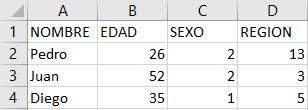
\includegraphics[width=0.8\linewidth,]{EJEMPLOMALABASE} \end{center}

\begin{Shaded}
\begin{Highlighting}[]
\NormalTok{Mal_ejemplo <-}\StringTok{ }\KeywordTok{read_excel}\NormalTok{(}\StringTok{"EJEMPLOMALABASE.xlsx"}\NormalTok{)}
\NormalTok{sjPlot}\OperatorTok{::}\KeywordTok{view_df}\NormalTok{(Mal_ejemplo)}
\end{Highlighting}
\end{Shaded}

Data frame: Mal\_ejemplo

ID

Name

Label

Values

Value Labels

1

NOMBRE

\textless output omitted\textgreater{}

2

EDAD

range: 26-52

3

SEXO

range: 1-2

4

REGION

range: 3-13

Además de que las bases de datos se encuentren bien estructuradas es importante que las etiquetas de las variables y las categorías se encuentren codificadas en ``UTF-8'' para que las letras puedan ser interpretadas por algunos softwares. Además de tener este tipo de codificación, es necesario que las bases de datos no posean tildes ni signos especiales (p.~ej ¿ " , ;), preferentemente solo dígitos alfanuméricos. De lo contrario se generan problemas de codificación que resultan en errores visibles como los que se presentan a continuación.

\begin{Shaded}
\begin{Highlighting}[]
\NormalTok{EncuestaCEPjul <-}\StringTok{ }\KeywordTok{read_sav}\NormalTok{(}\StringTok{"EncuestaCEPjul.sav"}\NormalTok{)}
\NormalTok{Encuesta_CEP <-}\StringTok{ }\KeywordTok{select}\NormalTok{(EncuestaCEPjul, SV1, MB_P2, ELE_}\DecValTok{7}\NormalTok{_}\DecValTok{1}\NormalTok{)}
\NormalTok{sjPlot}\OperatorTok{::}\KeywordTok{view_df}\NormalTok{(Encuesta_CEP, }\DataTypeTok{encoding =} \StringTok{"UTF-8"}\NormalTok{)}
\end{Highlighting}
\end{Shaded}

Data frame: Encuesta\_CEP

ID

Name

Label

Values

Value Labels

1

SV1

Considerando todas las cosas, ¿cuán satisfechoestá usted con su vida en este momento?

1108899

Totalmente insatisfechoTotalmente satisfechoNo sabeNo contesta

2

MB\_P2

¿Cómo calificaría Ud. la actual situacióneconómica del país?

1234589

Muy malaMalaNi buena ni malaBuenaMuy buenaNo sabeNo contesta

3

ELE\_7\_1

Para cada actividad que le nombraré indique si Ud.la realiza frecuentemente, a veces, o nunca. Miraprogramas políticos en televisión

12389

FrecuentementeA vecesNuncaNo sabeNo contesta

Junto de la importancia de la estructura de la base de datos, las etiquetas y la codificación es necesario revisar algunos otros puntos sobre una base de datos sociales antes de subirla, como lo pueden ser el tema de la documentación necesaria o el tema de la privacidad, a continuación, haremos una revisión de los distintos temas que son importantes para la publicación de una base de datos.

El proceso de preparación por el cual se llega a una base bien etiquetada, bien codificad y anonima se denomina \textbf{curatoria}. Por ello, la curatoria de datos es fundamental antes de compartir una base de datos para que todos los usuarios de ella puedan comprender adecuadamente su contenido y trabajar con la menor cantidad de complicaciones.

\hypertarget{guuxeda-icpsr-sobre-calidad-de-datos.}{%
\subsubsection{Guía ICPSR sobre calidad de datos.}\label{guuxeda-icpsr-sobre-calidad-de-datos.}}

Para resguardar al calidad de los datos cuantitativos ICPSR propone, entre otros, los siguientes puntos:

\hypertarget{errores-de-codificaciuxf3n}{%
\paragraph{Errores de codificación}\label{errores-de-codificaciuxf3n}}

Verifique cuidadosamente la coherencia entre las respuestas del cuestionario y los valores en la base de datos para el primer 5 a 10 por ciento de los registros de datos creados y luego elija registros aleatorios para controles de calidad. Posteriormente, puede realizar analisis descriptivos de distribución para evaluar si existen valores atipicos atribuibles a errores de codificación (p ej. 66 en la variable hijos en ves de 6). El uso de computadores y programas de encuesta y codificación puede ayudar a disminuir estos errores.

\hypertarget{recodificaciuxf3n-automatica}{%
\subparagraph{Recodificación automatica}\label{recodificaciuxf3n-automatica}}

Deje que la computadora realice codificaciones y rectificaciones complejas si es posible. Por ejemplo, para crear un serie de variables que describen la estructura familiar, escriba un código de computadora para realizar la tarea.
Los códigos de computadora no solo son precisos si las instrucciones son precisas, sino que también pueden
también se puede cambiar fácilmente para corregir un error lógico o de programación. Incluya en la documentación los codigos utilizados para la recodificación.

\hypertarget{consistencia}{%
\subparagraph{Consistencia}\label{consistencia}}

Evalue la coherencia entre las variables, identificando a quienes poseen convinaciones incoherentes. Por ejmplo, si alguien señala que su hijo no asiste a la escuela y luego responde preguntas sobre la escuela.

\hypertarget{identificadores-individuales-y-grupales}{%
\paragraph{Identificadores individuales y grupales}\label{identificadores-individuales-y-grupales}}

Proporcione variables identificadoras suficientes. Es fundamental que cada sujeto posea un id, además si la encuesta es longitudinal se puede proporcionar, junto al id de encuestado, un id por cada ocación que contesta la encuesta. Otros identificadores dependen del tema del estudio, por ejemplo, si se trabaja con escuelas, verifique que cada escuela tiene un identificador id-escuela. Si trabaja con encuestados de modo tal que dos o más son de la misma familia y cada encuestado corresponde a un nucleo familiar, indique un id para familia.

\hypertarget{nombres-de-variables}{%
\paragraph{Nombres de Variables}\label{nombres-de-variables}}

El nombre de la variable sera con lo que más se trabajara con los datos, por ende deben ser claros y utilizables por disintintos softwares.

Existen distintos estandartes para elegir los nombres de las variables.

\begin{enumerate}
\def\labelenumi{\arabic{enumi}.}
\item
  El primero consiste asignar un numero único anteponiendo una V de modo tal que, siendo n el numero de variables, las variables se nombran como Vn según su posición (p ej. V0001, v0002,\ldots Vn). Se antepone la V por que los software en general no permiten nombres de variables con solo caracteres números.
\item
  El segundo modo utiliza letras y números para agrupar las variables según escalas o temas (p.~ej Q1,Q2a,Q2b), si bien es un sistema que entrega más información, no informa sobre el contenido.
\end{enumerate}

3.El tercero consiste en utilizar abreviaturas nemotecnicas, es decir, nombres cortos de variables que representan el significado sustantivo de las variables facilitando su memorización y comprensión. Por ejemplo \emph{educpadr} como ``Educación del Padre''. Este tipo de nombres podrian ayudar a disminuir los errores en los análisis producidos por agregar una variable incorrecta en el código. El problema es que con la limitación de caracteres de los software es difícil generar abreviaturas arbitrarias que sean ampliamente reconocibles por un publico diverso.

\begin{enumerate}
\def\labelenumi{\arabic{enumi}.}
\setcounter{enumi}{3}
\tightlist
\item
  El cuarto consiste en Abreviaciones compartidas y registradas. Un sistema de raices y sufijos. Por ejemplo, todas las variables que tienen que ver con la educación pueden tener la raíz ED, y podria expresarse ``Educación del Padre'' como FAED, siendo estas nomesclatura previamente documentada. Esto implica una planificación previa y capacidad de organización para compartir las abreviaturas, así como herramientas para facilitar el encontrar las abreviaturas correctas en la biblioteca o documento de sufijos y prefijos.
\end{enumerate}

En consideración de estas opciones expuestas por ICPSR, se recomienda utilizar la tercera, puesto que cumple con la cualidad de la primera y la segunda de identificar las variables de modo único, a la vez que cumple con el criterio de hacer más comprensible y facil de recordar.

Junto a lo señalado por ICPSR, consideramos que al crear un nombre de la variable este debe ser utilizable por los distintos sofwares comunmente utilizados como SPSS, STATA y R. En vista de lo anterior sugerimos:

\begin{itemize}
\item
  Dos variables no pueden tener el mismo nombre
\item
  No utlizar más de 12 caracteres en el nombre
\item
  Empezar con una letra
\item
  Deben ser solo alfanuméricos (Numeros y letras, sin símbolos . ; , : `` \$ @)
\item
  En minúscula
\item
  No utilizar la letra ñ, remplazarlo por gn (agnos, en vez de años)
\item
  Remplazando espacios por guionbajo. (edad\_rec)
\end{itemize}

\hypertarget{etiquetas-de-variables}{%
\subparagraph{Etiquetas de variables}\label{etiquetas-de-variables}}

las variables deben ser correctamente etiquetadas. Las etiquetas deben partir con el numero del item en el cuestionario para poder asociarlo. Luego debe darse información sobre el contenido de la variable o ingresar directamente la pregunta realizada al encuestado.

Considerando las limitaciones de caracteres de los sofwares, en base a manuales universitarios de SPSS y STATA, se sugiere que las etiquetas de las variables no superen los 120 caracteres.

\hypertarget{codificaciuxf3n}{%
\paragraph{Codificación}\label{codificaciuxf3n}}

\begin{itemize}
\item
  Variables de identificación. Proporcione campos al comienzo de cada registro para acomodar todas las variables de identificación. Las variables de identificación a menudo incluyen un número de estudio único y un número de encuestado para representar cada caso.
\item
  Categorías de código. Las categorías de códigos deben ser mutuamente excluyentes, exhaustivas y estar definidas con precisión. Cada respuesta de la entrevista debe encajar en una y solo una categoría. La ambigüedad provocará dificultades de codificación y problemas con la interpretación de los datos.
\item
  Conservación de la información original. Codifique tantos detalles como sea posible. Registrar datos originales, como edad e ingresos, es más útil que colapsar o poner entre corchetes la información. Con datos originales o detallados, los analistas secundarios pueden determinar otros paréntesis significativos por sí mismos en lugar de limitarse a los elegidos por otros.
\item
  Preguntas cerradas. Las respuestas a las preguntas de la encuesta que están precodificadas en el cuestionario deben conservar este esquema de codificación en los datos legibles por máquina para evitar errores y confusiones.
\item
  Preguntas de final abierto. Para los ítems abiertos, los investigadores pueden usar un esquema de codificación predeterminado o revisar las respuestas iniciales de la encuesta para construir un esquema de codificación basado en las categorías principales que surgen. Cualquier esquema de codificación y su derivación deben informarse en la documentación del estudio.
\item
  Respuestas codificadas por el usuario. Cada vez más, los investigadores envían el texto completo de las respuestas a las preguntas abiertas a los archivos para que los usuarios puedan codificar estas respuestas ellos mismos. Debido a que dichas respuestas pueden contener información confidencial, deben ser revisadas por riesgo de divulgación y, si es necesario, tratadas por archivos antes de su publicación.
\item
  Comprobar codificación. Es una buena idea verificar o verificar el código de algunos casos durante el proceso de codificación, es decir, repetir el proceso con un codificador independiente. Por ejemplo, si se asigna más de un código a la respuesta de una entrevista, esto resalta problemas o ambigüedades en el esquema de codificación. Esta codificación de verificación proporciona un medio importante de control de calidad en el proceso de codificación.
\item
  Serie de respuestas. Si una serie de respuestas requiere más de un campo, organizar las respuestas en clasificaciones importantes significativas es útil. Respuestas dentro de cada especialidad categoría se les asigna el mismo primer dígito. Los dígitos secundarios pueden distinguir específicos respuestas dentro de las categorías principales. Tal esquema de codificación permite el análisis de la datos utilizando agrupaciones amplias o categorías más detalladas.
\end{itemize}

\hypertarget{identificar-casos-perdidos}{%
\paragraph{Identificar Casos perdidos}\label{identificar-casos-perdidos}}

ICPSR no establece un modo determinado de identificar los perdidos aunque señala las ventajas y desventajas de distintos tipos de codificación. Igualmente sugiere distintos tipos de perdidos que deben ser identificados. Cabe destacar que como regla general para la preservación, los perdidos se deben codificar del modo más similar a las categorias de las variables, de modo tal que una variable numerica de un digito se indica con (8,9) y una variable categorica con alternativas de texto con (``No sabe'', ``No responde'')

\begin{itemize}
\item
  Rechazo / Sin respuesta. El sujeto se negó explícitamente a responder una pregunta o no la respondió cuando debería haberlo hecho.
\item
  No lo sé. El sujeto no pudo responder una pregunta, ya sea porque no tenía una opinión o porque la información requerida no estaba disponible (por ejemplo, un encuestado no pudo proporcionar los ingresos familiares en dólares del año anterior).
\item
  Error de proceso. Por alguna razón, no hay respuesta a la pregunta, aunque el sujeto proporcionó una. Esto puede resultar de un error del entrevistador, codificación incorrecta, falla de la máquina u otros problemas.
\item
  No aplica. Al sujeto nunca se le hizo una pregunta por alguna razón. A veces, esto se debe a patrones de omisión después de preguntas de filtro, por ejemplo, a los sujetos que no están trabajando no se les pregunta sobre las características del trabajo. Otros ejemplos de inaplicabilidad son los conjuntos de elementos solicitados solo de submuestras aleatorias y los solicitados a un miembro de un hogar pero no a otro.
\item
  Sin coincidencia. Esta situación surge cuando los datos se obtienen de diferentes fuentes (por ejemplo, un cuestionario de encuesta y una base de datos administrativa) y no se puede localizar la información de una fuente.
\item
  Datos no disponibles. La pregunta debería haberse formulado al encuestado, pero por un por otro motivo distinto de los enumerados anteriormente, no se dio ni registró ninguna respuesta.
\end{itemize}

Considerando las ventajas y desventajas de las distintas formas de codificación se sugiere a titulo personal utilizar valores perdidos con valores altos en negativo de modo tal que sean estandar para todas las variables y no sean confundible con los valores posibles de dichas variables. Se propone utilizar los siguientes valores perdidos, usando numericos o caracteres segÚn corresponda.

\begin{longtable}[]{@{}ll@{}}
\toprule
Código de texto & Código numérico\tabularnewline
\midrule
\endhead
No responde & -999\tabularnewline
No sabe & -998\tabularnewline
Error de Proceso & -997\tabularnewline
No aplica & -996\tabularnewline
Sin coincidencia & -995\tabularnewline
No disponible & -994\tabularnewline
\bottomrule
\end{longtable}

Para obtener información adicional sobre datos georeferenciados e imputaciones revise directamente la guía ofrecida por ICPSR disponible en este \href{https://www.icpsr.umich.edu/files/deposit/dataprep.pdf}{vinculo}

\hypertarget{documentar}{%
\section{\texorpdfstring{\textbf{Documentar:}}{Documentar:}}\label{documentar}}

Existen distintos estándares sobre que información incorporar junto con los datos destacando la importancia de que estos materiales sean legibles por humanos y por inteligencia artificial \citep{go_fair}. A continuación se presenta un mínimo de los documentos necesarios para publicar los datos basado en la propuesta de Marwick \citep{dandrea_Meetup_2020}.

\begin{center}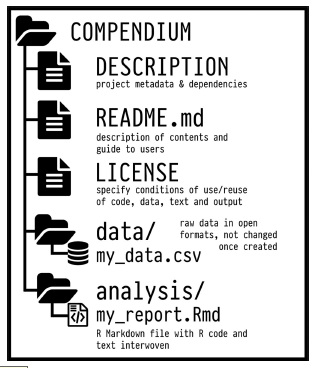
\includegraphics[width=0.5\linewidth,]{images/small_rc} \end{center}

Además de estos documentos, como se muestra en la imagen siguiente se recomienda incorporar metadatos para que los datos sean utilizables por inteligencia artificial (Cumpliendo con criterios FAIR) y libros de códigos (Nombre de las Variables) para que investigadores se familiaricen con el contenido \citep{tierney_Realistic_2020}. Incorporar los metadatos y el libro de códigos es fundamental para cumplir con los principios FAIR, ya que permite que los datos sean faciles de encontrar para herramientas de búsqueda mediante conceptos clave y facilita la posibilidad de reutilización de los datos mediante una buena documentación que facilite su uso.

\begin{center}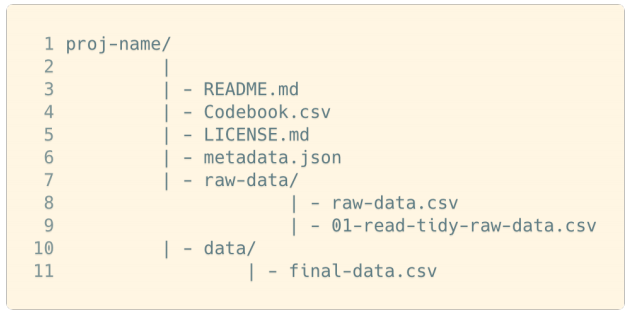
\includegraphics[width=0.5\linewidth,]{images/esquemadedatos} \end{center}

Como puede notarse estos estándares tienen mayor afinidad para los datos cuantitativos, no obstante, la descripción del proyecto, el readme con la información que contienen los datos, la licencia y un libros de preguntas, podrían ser de mucha utilidad para un investigador que se aproxima por primera vez a un conjunto de entrevistas, del mismo modo incorporar los análisis realizados por el equipo de investigación seria de utilidad para un nuevo equipo de investigación que pretenda trabajar con estos datos cualitativos.

En consideración de lo anterior es necesario hacer algunos cambios a estos esquemas. A continuación se propone un conjunto de documentos comunes que deben estar incluidos, junto con una guía de como escribirlos en formato abiertos para cumplir con las recomendaciones del libro Managing and sharing research data: a guide to good practice \citep{corti_Managing_2019}. Cabe destacar que los formatos abiertos se contraponen a los formatos propietarios para los cuales se requieren legalmente licencias pagadas como Word.docx.

\hypertarget{readme}{%
\subsubsection{Readme}\label{readme}}

El readme es un documento que debe responder las siguientes preguntas sobre la producción de la información \citep{tierney_Realistic_2020}.

\begin{itemize}
\item
  Quién produjo la información
\item
  Cual es el contenido de los datos
\item
  Cuando fue producida la información
\item
  Dónde fue recolectada
\item
  Por qué se recopiló
\item
  Cómo se recopiló
\end{itemize}

Para crear este documento se suele utilizar el formato y lenguaje Markdowm de extencion .md, este formato posee la ventaja de no ser un formato propietario que permite incluir de modo sensillo distintos elementos ultiles como los links las imagenes y las tablas. Le recomendamos realizar la escritura en este formato, para ello se puede escribir el documento en R Studio señalando como extensión .md o para quienes no manejen el softweare, pueden crear el documento en la pagina \href{https://dillinger.io/}{Dillinger}. A continuación presentamos los pasos mínimos para crear el documento.

En primer lugar al acceder a la pagina Dillinger, encontrara una entrada de texto señalada como sector A y una salida con imágenes, enlaces y otros recursos posibles de Markdowm. Este tipo de lenguaje busca ser la forma más simple para los usuarios de dar formato a sencillas paginas web. Para generar un texto mínimo simplemente debe borrar el contenido en el sector y escribir un breve documento que responda las preguntas señaladas por \citep{tierney_Realistic_2020}. Para borrar fácilmente el contenido sugiero apretar el botón para ampliar el sector A y seleccionar todo el texto con el cursor (o con ctrl + a, habiendo hecho click en el texto).

Si desea agregar títulos, imágenes o enlaces puede utilizar los ejemplos de la pagina o aprender lo basico en la pagina de \href{https://markdown.es/sintaxis-markdown/}{Markdowm}, la cual contiene un breve vídeo y una sucinta guía.

Además es fundamental incorporar en el README un esquema de los documentos presentes en la carpeta, incluyendo cada archivo en su respectiva carpeta.

\begin{center}\includegraphics[width=1\linewidth,]{images/Sin título} \end{center}

\hypertarget{licencia}{%
\subsection{Licencia}\label{licencia}}

La licencia se puede crear fácilmente al publicar los datos en OSF. En la siguiente sección se señala como hacerlo.

\hypertarget{metadatos}{%
\subsection{Metadatos}\label{metadatos}}

La creación de los metadatos requiere previamente que se cree el identificador y la pagina web en osf que almacenara los datos. Por ello la creación de los metadatos sera posterior a la publicación. Cabe destacatar que el modo de creear metadatos difiere segun si el tipo de material es una transcripción de entrevista en PDF o una base de datos en formata sav, stat o rda.

\url{https://www.sejda.com/es/edit-pdf-metadata}

\hypertarget{documentos-especiales-seguxfan-tipo-de-metodologuxeda}{%
\subparagraph{Documentos especiales según tipo de metodología}\label{documentos-especiales-seguxfan-tipo-de-metodologuxeda}}

Para publicar datos cuantitativos se recomienda recopilar y producir los siguientes materiales con el objetivo de que los usuarios de la base de datos cuenten con información suficiente para utilizarla correctamente. Los siguientes documentos deben ser subidos en PDF y Blog de notas.txt con codificación utf8.

\begin{itemize}
\tightlist
\item
  Cuestionario
\item
  Consentimiento informado
\item
  Libro de códigos
\item
  Ficha técnica
\item
  Manual de usuario
\item
  Descriptivos (Optativo)
\item
  Publicaciones asociadas a los datos (Optativo)
\item
  Descripción e información detallada para metadatos.
\end{itemize}

Para publicar datos cualitativos se sugiere documentar la siguiente información.

• Transcripciones

• registros audiovisuales (De ser necesario)

• Investigar métodos y prácticas que estén completamente documentados

• Copia en blanco del formulario de consentimiento informado con el número de aprobación del IRB

• Detalles sobre el escenario de las entrevistas

• Detalles sobre la selección de los sujetos de la entrevista

• Instrucciones dadas a los entrevistadores

• Instrumentos de recopilación de datos como cuestionarios de entrevistas

• Medidas tomadas para eliminar identificadores directos en los datos (por ejemplo, nombre, dirección, etc.)

• Cualquier problema que surgió durante el proceso de selección y / o entrevista y cómo se manejaron

• Lista de entrevistas

\hypertarget{publicar}{%
\section{\texorpdfstring{\textbf{Publicar}}{Publicar}}\label{publicar}}

\hypertarget{osf-y-plataformas-para-publicar-datos}{%
\subsection{OSF y plataformas para publicar datos}\label{osf-y-plataformas-para-publicar-datos}}

La plataforma web Open Science Framework (OSF) ofrece gratuitamente servicios de infraestructura digital que permite un espacio de registro para las distintas etapas de un proyecto de investigación. Actualmente existen otras plataformas con objetivos similares como Zenovo, Mendeey, Figshare, Dryad o icpsr, y si bien todas son buenas herramientas, se remienda utilizar OSF por diversos motivos señalados por \citet{kryvokhyzha_best_2019} y un documento informativo de la Librería de Universidades de la Universidad de OKLAHOMA \citet{bibliotecasuniversitarias_Make_2020}. En primer lugar, a diferencia de Dryad, OSF es una plataforma gratuita, con mejor estructura de repositorios y con posibilidades de corregir errores. En segundo lugar, figshare la capacidad de estructurar los repositorios en distintos componentes, no esta optimizado para descargar muchos archivos a la vez y, además es una empresa con fines de lucro. Por su parte OSF, permite estructurar de diversos modos los repositorios, esta optimizado para descargas y es una organizaicon sin fines de lucro que es financiada por el Centro para la Ciencia Abierta \href{https://www.cos.io/}{cos} con recursos para 50 años más. En tercer lugar, a diferencia de Zenovo OSF si cuentan con estadisticas de descarga que nos permiten evaluar la visibilidad de los datos. No obstante, si el equipo investigador lo considera conveniente podria subir sus datos a multiples plataformas. En esta linea, además de osf, recomendamos almacenar los datos paralelamente en \href{https://www.openicpsr.org/openicpsr/workspace?path=openICPSR}{OpenICPSR} puesto que esto permitira conectar nuestros datos con el buscador de ICPSR, el cual tiene amplia visibilidad dentro del campo de las ciencias sociales a nivel internaciónal.

Un usuario de esta página puede crear repositorio denominado proyecto, el cual puede contener a su vez componentes que pueden ser investigaciones o datos específicos dentro del proyecto. Se pueden crear más componentes de estos tipos dentro de los componentes del proyecto. Esta estructura permite almacenar conjuntamente trabajos relacionados.

La página promueve que se registren productos de la investigación de las distintas etapas del proceso. En primer lugar posee un espacio para los ``pre-registros'' que son un documento en el cual se expone brevemente el diseño de la investigación, las hipótesis y la metodología, lo cual aumenta la rigurosidad de las investigación.

Ambas evaluaciones de osf señalan que un problema es el limite de almacenamiento de oslo 5gb por archivo. Este limite ha sido miodificado el 5 de novimiebbre del 2020, agregando un limite de 5gb a los proyectos que esten privados y 50 a los publicos. No obstante, el problema del espacio se puede resolver conectando osf con otros servicios de almacenamiento con mayor capacidad.

\hypertarget{pasos-para-publiar}{%
\subsubsection{Pasos para publiar}\label{pasos-para-publiar}}

\begin{enumerate}
\def\labelenumi{\arabic{enumi}.}
\setcounter{enumi}{-1}
\tightlist
\item
  Crear una cuenta en OSF.
\end{enumerate}

Para crear una cuenta en OSF diríjase a este \href{https://osf.io/register?campaign=\&next=https\%3A\%2F\%2Fosf.io\%2F\&view_only=}{link}

\begin{enumerate}
\def\labelenumi{\arabic{enumi}.}
\tightlist
\item
  Crear un repositorio de los datos
\end{enumerate}

Para que los datos puedan contar con un identificador y ser faciles de encontrar , se deben sebir en un repositorio, para ello se debe crear uno seleccionando dicha opción en la pagina de OSF como se señala en la imagen. Indique el nombre del proyecto y establezca la localización (Esta no debe ser necesariamente el lugar donde usted se encuentra)

\begin{center}\includegraphics[width=0.5\linewidth,]{images/crearrepo} \end{center}

2.Indicar contenido

Si solo se subirán los datos cambie la cateogira desde proyecto a datos, como se indica en la siguiente imagen.

\begin{center}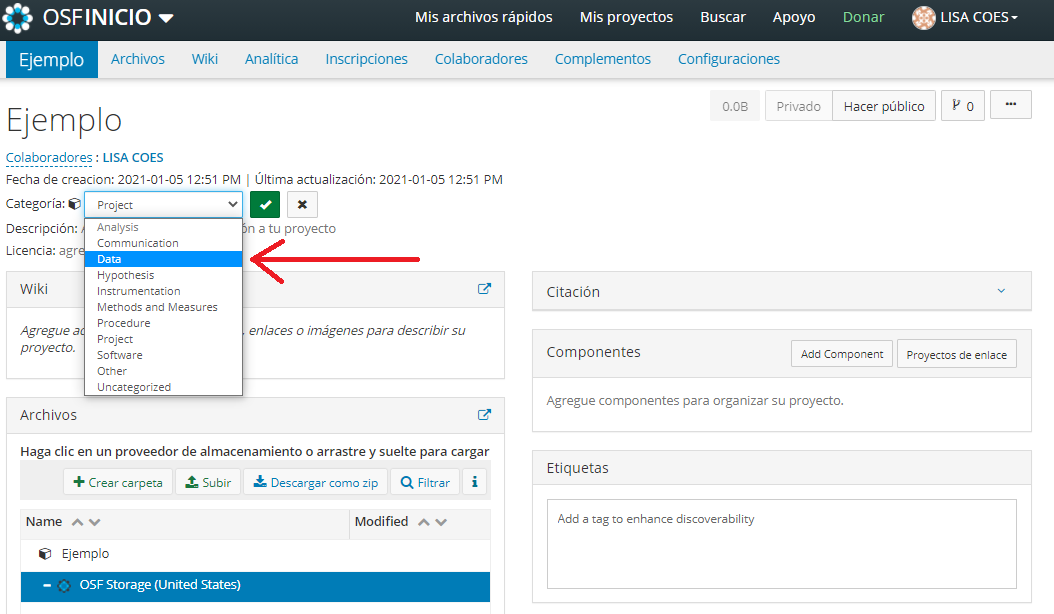
\includegraphics[width=0.5\linewidth,]{images/cambiaradatos} \end{center}

\begin{enumerate}
\def\labelenumi{\arabic{enumi}.}
\setcounter{enumi}{2}
\tightlist
\item
  Subir datos y documentos.
\end{enumerate}

Suba los documentos creados en ``Documantar''. Para ello debe seleccionar la localización (paso 1) y luego seleccionar ``subir'' (paso 2). Con ello apareceran los documentos de su ordenador, y debera seleccionar y subir los archivos necesarios. Tambien puede crear carpetas para ordenar los documentos.

\begin{center}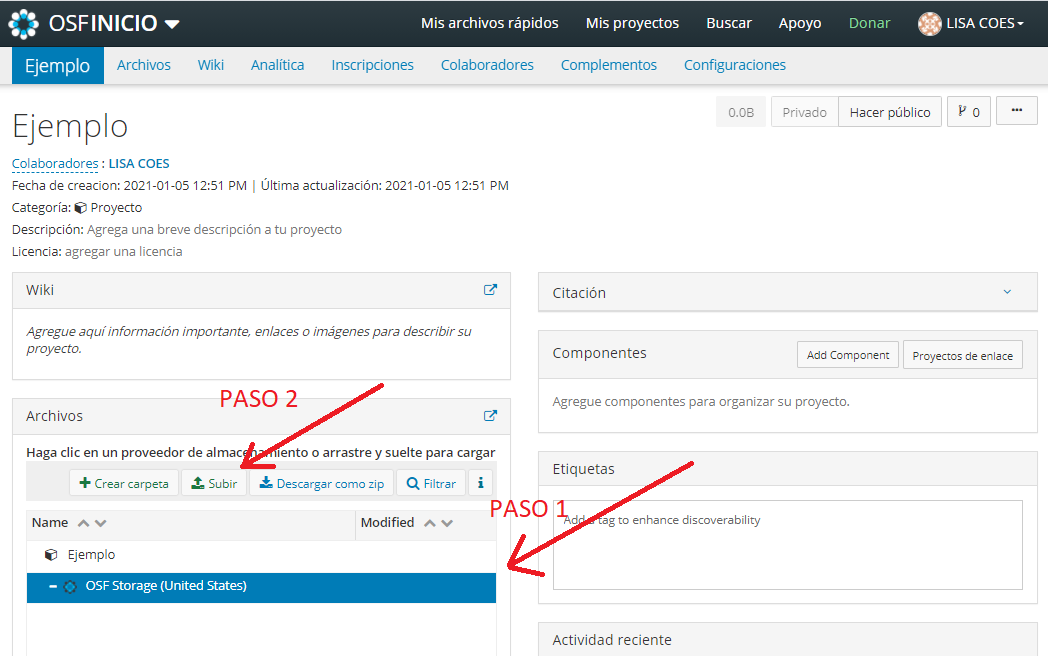
\includegraphics[width=0.5\linewidth,]{images/subirdatos} \end{center}

\begin{enumerate}
\def\labelenumi{\arabic{enumi}.}
\setcounter{enumi}{3}
\tightlist
\item
  Agregar información.
\end{enumerate}

OSF ofrece varios modos para dar más información sobre sus datos. Le suguerimos rellenar las palabras claves del proyecto, haciendo alusión al contenido de las preguntas, el área temática, los sujetos de estudio y lo que considere necesario.

Describa el contenido y la estructura de los documentos en ``Wiki''.

Tambíen una descripción más breve en descripción.

\begin{enumerate}
\def\labelenumi{\arabic{enumi}.}
\setcounter{enumi}{4}
\tightlist
\item
  Crear licencia.
\end{enumerate}

En base a las recomendaciones revisadas recomendamos utilizar una licencia CCO, como se indica en la imagen. Seleccione add license y se abrirá una lista de opciones. Seleccione la sugerida o la que considere pertinente.

\begin{enumerate}
\def\labelenumi{\arabic{enumi}.}
\setcounter{enumi}{5}
\tightlist
\item
  Crear DOI
\end{enumerate}

Para poder crear un doi es necesario que los datos se encuentren en modo ``publico''. Para ello seleccione ``Make Public'' en la esquina superior derecha. Solo cuando los datos sean públicos OSF ofrecerá la opción de agregar un identificador, para ello solo seleccione ``add doi''.

\begin{enumerate}
\def\labelenumi{\arabic{enumi}.}
\setcounter{enumi}{6}
\tightlist
\item
  Almacenar local.
\end{enumerate}

Deje la carpeta con la documentación y los datos en ordenadores que sean de la organización a la que participa. Tambien, puede consultar a la biblioteca de su universidad si es posible que almacenen sus datos para tener una copia de seguridad. Con ello se fomenta que los datos sean perdurables cumpliendo con los criterios de ICSU y con las recomendaciones de la tuberia de datos de ICPSR.

\hypertarget{crear-metadatos-para-datos-cualitativos-o-cuantitativos.}{%
\paragraph{Crear Metadatos para datos cualitativos o cuantitativos.}\label{crear-metadatos-para-datos-cualitativos-o-cuantitativos.}}

\textbf{Paso 1}

Para crear los metadatos de forma muy sencilla se puede utilizar un archivo csv, que se puede editar con el programa Excel o cualquier Hoja de calculo. A continuación entregamos un link para descargar un csv con los campos para rellenar los metados, cumpliendo con los campos utilizados por Dataverse Harvar y los ``Social Science and Humanities Metadata'' de ICPSR.

Para crear los metadatos usted solo debe escribir en las casillas de abajo de las categorias, la respuesta para cada uno de los campos, señalando el identificador, el Titulo de los datos, los autores, entre otros. Es necesario que rellene los campos en ingles. Con una traducción simple de \href{https://translate.google.com/}{Google Traductor} o \href{https://www.deepl.com/es/translator}{Deepl} es suficiente.

Para descargar el archivo csv editable en Excel seleccione \href{https://raw.githubusercontent.com/franciscomeneses/CADIS/master/metadata.csv}{Descargar Metadata.cvs}. Si no le ofrece directamente abrirlo con Excel, puede apretar click derecho sobre el archivo, seleccionar ``Abrir con'', luego Excel, si no aparece seleccionamos ``Elegir otra aplicación'', ``Más aplicaciones'' y luego Excel.

A continuación le presentamos una tabla con cada uno de los campos que debe llenar y con que debe rellenarlos. Despues de agregar la información a los metadatos solo guarde el documento desde excel, y este se guardara automaticamente en csv delimitado por Semi-coma (;) en codificación UTF-8 (Que permite incorporar comas a los metadatos)

Cabe destacar que para el primer campo correspondiente al Identificador antes del codigo entregado por OSF, debe estar escrito \url{https://doi.org/} como se muestra en el documento descargado. Esto es para cumplir con los estandares FAIR.

\textbf{Paso 2}

Despúes de haber creado el documento csv con nuestra información solo debemos seleccionar al siguiente link e ir al sitio web: \href{https://csvjson.com/csv2json}{csvjson.com}. En este citio tenemos que apretar Select a file\ldots{} y buscar el documento csv creado. Posteriormente, se debe señalar output: ``Array'' y ``Minify'', como se señala en la imagen. Con estas opciónes apretamos el boton morado \textgreater Convert bajo el cuadrado que posee nuestro documento CSV. Cuando este listo apretamos el botón Download, como se señala en la Imagen. El documento se descargara con el nombre csvjson, debe cambiarlo a metadata.

\begin{center}\includegraphics[width=0.5\linewidth,]{images/crearrepo} \end{center}

\textbf{Paso 3}

Finalmente debemos agregar los archivos csv y json al repositorio, recuerde cambiar el nombre del documento a metadata.

\hypertarget{mejorar-metadatos-del-libro-de-codigos-para-datos-cuantitativos}{%
\paragraph{Mejorar metadatos del Libro de codigos (Para datos cuantitativos)}\label{mejorar-metadatos-del-libro-de-codigos-para-datos-cuantitativos}}

Para el libro de códigos recomendamos utilizar \href{https://opencpu.psych.bio.uni-goettingen.de/ocpu/library/codebook/www/}{Codebook Generator}. En esta plataforma basta con seleccionar una base de datos, apretar generate codebook y descargar para tener un libro de códigos. Sugerimos además, para seguir los estandares FAIR cambiar la linea de codigo 51 por las lineas de código señaladas más adelante, antes de generar el libro de codigos. En estos codigos usted debe agregar la información de los matadatos entre las "" usted puede agregar el nombre de su base de datos, el doi, los autores y las palabras clave. Recuerde que el DOI se creara despues de publicada la base por ello recomendamos hacer el libro de codigos despues de crear el repositorio en osf, además antes del DOI hay que anteponer \url{https://doi.org/} para que funcione como un link a nuestro proyecto.

Para obtener como citar su documento busque en su repositorio de OSF ``citation'' y despliege la ventana, le aparecerán citas en distintos formatos.

metadata(codebook\_data)\(name <- "Nombre de su base de datos" metadata(codebook_data)\)doi \textless- ``\url{https://doi.org/10.17605/OSF.IO/VC8YU}''
metadata(codebook\_data)\(keywords <- c("Palabra clave 1", "Palabra clave 2","Palabra clave 3","Palabra clave 4" ) metadata(codebook_data)\)authors \textless- c(``Autor 1'', ``Autor 2'',``Autor 3'')
metadata(codebook\_data)\$cite \textless- ``Meneses, F. J. (2020, December 2). Bases. \url{https://doi.org/10.17605/OSF.IO/VC8YU}''

\hypertarget{mejorar-metadatos-para-documentos-pdf-de-transcripcion-para-datos-cualitativos}{%
\paragraph{Mejorar metadatos para documentos PDF de transcripcion (Para datos Cualitativos)}\label{mejorar-metadatos-para-documentos-pdf-de-transcripcion-para-datos-cualitativos}}

Para mejorar los metadatos podemos incrustar más metadatos en los documentos PDF, en las transcripciones por ejemplo, de modo muy sencillo. Para ello debemos ir a la pagina \href{https://www.sejda.com/edit-pdf-metadata}{Sejda.com}. En esta pagina basta con apretar Upload PDF file, para que nos entregue un conjunto de casillas para rellenar con información sobre la fecha de producción y los autores del documento. Lamentablemente no ofrece un espacio para incorporar el DOI creado en OSF, no obstante, aconsejo incorporar el DOI ya sea en autor, creador o productor. Al pegar el DOI en la casilla debe anteponer \url{https://doi.org/} para que el DOI funcione como un link a nuestro proyecto.

\hypertarget{almacenamiento-y-curatoria}{%
\chapter{Almacenamiento y Curatoria}\label{almacenamiento-y-curatoria}}

\begin{quote}
¿Qué es la Curatoría y como se relaciona con la accesibilidad de los productos de investigación?
\end{quote}

El objetivo final de esto es que usted en el futuro, investigadores, estudiantes o público en general, puedan buscar en un repositorio un tema de interés como ``Socialización escolar'' y con ello acceder fácilmente a distintas bases de datos, transcripciones de entrevistas y experiencias de investigaciones sobre la temática, haciendo más eficiente e informadas las investigaciones. Esto permitirá unas ciencias sociales más rigurosas, más colaborativas y con una preservación capas de acumular evidencia para futuros estudios históricos.

Para poder garantizar un proceso adecuado del almacenamiento de productos de investigación, es necesario alcanzar una buena curatoría, la cual depende de un conjunto de factores. Entre estos factores destacan:

\begin{itemize}
\item
  \textbf{Buenos ``datos''}. Aunque el concepto se asocia con lo cuantitativo, en este documento nos referimos con dicho termino al conjunto de materiales que son producidos por los proyectos de investigación mediante técnicas de recolección/producción de información que sirven posteriormente para el análisis cualitativo y/o cuantitativo (p.~ej. entrevistas, encuestas, transcripciones, recopilaciones). De hecho, los dos repositorios cualitativos más famosos de transcripciones de entrevistas y focus groups (QualiData y QDR) utilizan el termino datos para referirse a esta información producida por investigaciones. Abrir buenos datos al público, significa que estos materiales pueden ser utilizados, comprendidos y trabajados por distintos tipos de investigadores. Esto sin duda implica un esfuerzo por parte de los investigadores a la hora de producir información para asegurar que quede registrada de modo tal que sea accesible y fácil de encontrar para quien la quiera.
\item
  \textbf{Metadatos precisos}. Los metadatos son información de los datos que permiten comprender cuál es su contenido y su posible utilidad. Por ejemplo, nombre del material, tipo de material, como fue producida esa información, cual fue la institución e investigadores encargados de su producción, entre otros. Junto con esta descripción de distintos aspectos, se consideran dentro de las ciencias sociales como documentación relevante los manuales de usuario, pautas de entrevistas, bitácoras o cualquier documento que ayudo a la producción de la información o ayuda a ser comprendida.
\item
  \textbf{Infraestructura Digital}. Refiere a las páginas web, y las herramientas digitales que puedan ayudar a organizar, localizar y distribuir los datos de las investigaciones. Por ejemplo, es necesario contar con buscadores en los repositorios de materiales de investigación, estos deberían permitir encontrar todas las bases de datos de encuestas y todas las transcripciones de entrevistas que estén asociados a un término de búsqueda como ``desigualdad de género'' y sus sinónimos. Una herramienta de este tipo de fácil uso, puede ser un gran aporte a las investigaciones de las ciencias sociales.
\item
  \textbf{Organización y practicas abiertas}: Para que un servicio de almacenamiento de datos funcione adecuadamente debe existir actitudes, conocimientos y practicas colectivas por parte de los investigadores en torno a cómo y por qué almacenar sus datos abiertamente. Del mismo modo, son necesarios algunas personas dedicadas a la administración de los repositorios en línea y a la formación de los investigadores para adecuase al contexto digital.
\end{itemize}

En suma, para tener un buen almacenamiento de materiales sociales para investigar, que estén bien clasificados y sean faciles de encontrar, es necesario tener cierta infraestructura digital y procesos de curatoría. Igualmente, estos procesos pueden apoyar la mejora de la calidad de los datos y su difusión a distintos investigadores.

\hypertarget{estuxe1ndares-y-sugerencias-sobre-la-preservaciuxf3n-de-datos}{%
\chapter{Estándares y sugerencias sobre la preservación de datos}\label{estuxe1ndares-y-sugerencias-sobre-la-preservaciuxf3n-de-datos}}

Para poder generar una ciencia social más colaborativa y eficiente, es necesario que la comunidad de las ciencias sociales compartan estándares compartidos respecto a la calidad de los datos y del almacenamiento. De este modo los trabajos de investigación y los materiales de por si complejos serán más faciles de comprender y ser utilizados por terceros.

En la sección actual se revisarán tanto declaraciones de instituciones relacionadas con la Curatoría y el mantenimiento de los datos, como documentos que fijen normas comunes para el almacenamiento. El objetivo es recopilar y sistematizar los estándares de calidad para un repositorio abierto de datos. Posteriormente, evaluaremos distintos repositorios a partir de los criterios de la calidad sistematizados, buscando ventajas y desventajas de distintas experiencias en el almacenamiento de bases de datos de investigación social, junto con aquellos aprendizajes que puedan desprenderse.

El resultado final de este trabajo será una propuesta de almacenamiento acorde a los estándares internacionales y un manual que facilite a los usuarios seguir estos estándares.

A continuación se revisaran los siguientes estándares internacionales.

\begin{itemize}
\item
  Acceso abierto ICSU
\item
  FAIR
\item
  DMP
\item
  RISE-DDC
\item
  Tubería de datos ICSPR
\item
  OASIS - Research Managament Data.
\item
  Esquema CILAC.
\end{itemize}

\hypertarget{acceso-abierto-icsu}{%
\section{Acceso abierto ICSU}\label{acceso-abierto-icsu}}

El Consejo Internacional para la Ciencia \citep{icsu_Open_2014} defiende los siguientes objetivos para la apertura. El registro científico debe ser:

\begin{itemize}
\item
  libre de barreras financieras a las que pueda contribuir cualquier investigador;
\item
  libre de barreras financieras para que cualquier usuario acceda inmediatamente después de la publicación;
\item
  disponible sin restricción de reutilización para cualquier propósito, sujeto a
  atribución adecuada;
\item
  calidad garantizada y publicada de manera oportuna; y
\item
  archivado y disponible a perpetuidad
\end{itemize}

Para alcanzar estos objetivos \citet{ics_Open_2020} señala que las instituciones financiaras y las universidades deben fortalecer las capacidades para alinearse con los principios FAIR, los cuales presentamos a continuación.

\hypertarget{principios-fair-datos-metadatos-e-infraestructura-digital.}{%
\section{Principios FAIR: Datos, Metadatos e infraestructura digital.}\label{principios-fair-datos-metadatos-e-infraestructura-digital.}}

Los principios de almacenamiento FAIR (Findable, Accessible, Interoperable, Reusable), son ampliamente reconocidos a nivel mundial. Estos principios han sido promovidos por organizaciones científicas regionales como CILAC \citep{ramirez_Ciencia_2019} y Europeas \citep{ec_FAIR_2016}. En Chile ANID del ministerio de ciencias, ha señalado la política de acceso a datos que impulsará se guiara por los principios FAIR.

Los principios FAIR, son sumamente compatibles con las diversas formas de información producida por las ciencias sociales, ya sean documentos de texto, audiovisuales o bases de datos. Este es un buen motivo para fomentar los principios FAIR en todos los tipos de investigaciones en ciencias sociales.

El objetivo general de estos principios es que los productos de investigación estén disponibles en la web, de modo tal que puedan ser buscados directamente por investigadores o por inteligencia artificial \citep{gofair_FAIR_2020}. A continuación, se explican estos principios y como pueden ayudar a las ciencias sociales.

\begin{figure}[!ht]

{\centering 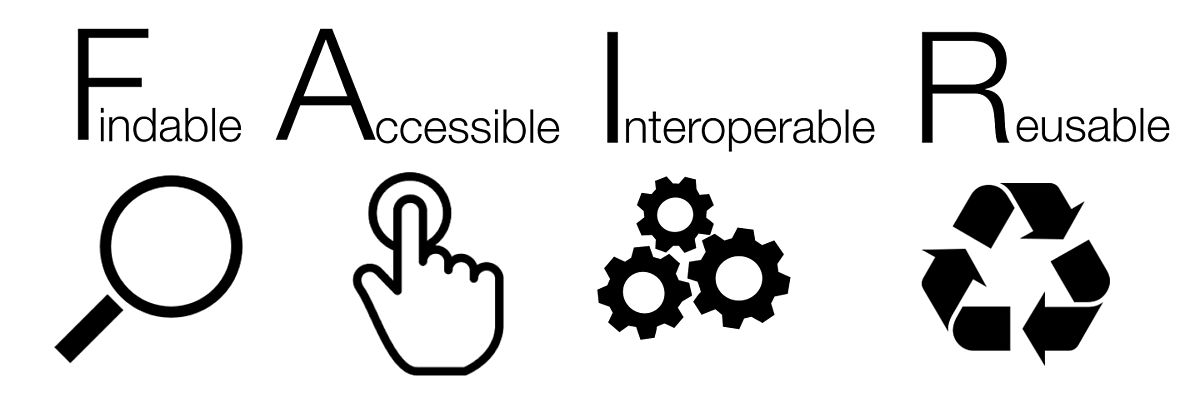
\includegraphics[width=0.8\linewidth,]{images/FAIR_data_principles} 

}

\end{figure}

Los principios se refieren a tres tipos de entidades: \emph{``datos''} (o cualquier producto de investigación como objeto digital), \textbf{``metadatos''} (información sobre ese objeto digital) e infraestructura digital (Capacidades y herramientas necesarias en repositorios web).

\hypertarget{findable-encontrables}{%
\subsection{\texorpdfstring{\textbf{Findable} \emph{(``Encontrables'')}}{Findable (``Encontrables'')}}\label{findable-encontrables}}

El primer paso para (re) usar datos es encontrarlos. Los metadatos y los datos deben ser fáciles de encontrar tanto para humanos como para computadoras. Los metadatos legibles por máquina son esenciales para el descubrimiento automático de conjuntos de datos y servicios, por lo que este es un componente esencial del proceso de FAIRification .

\begin{quote}
F1. A los datos se les asigna un identificador único y persistente a nivel mundial.
\end{quote}

Los identificadores únicos eliminan la ambigüedad, facilitando que una investigación, una base de datos o cualquier producto de investigación, no sea confundido con otro producto por tener un nombre o características similares.

Los ejemplos más comunes de identificadores son los URL (Localizador Uniforme de Recursos) los cuales asignan un sitio único a cada página web, como los URL ``www.google.com'' o ``www.youtube.com''. Otro tipo de identificadores más cercano a las ciencias sociales son los ISBN (Número Internacional Normalizado del Libro) o el DOI (Identificador de Material Digital) que solemos ver asociados a los artículos de investigación. A diferencia del URL el doi no cambia, aunque el material cambie de ubicación en la web. Así, los identificadores se asocian de forma única a los datos (Bases de datos, entrevistas, transcripciones), como es el ejemplo de este doi \url{https://doi.org/10.5064/F6HTXF0H} que corresponde al identificador de un conjunto de materiales y Focus Groups sobre género y participación en el desarrollo comunitario en Senegal.

Estos identificadores también ayudarán a que el trabajo sea más fácilmente compartido, reconocido y posea un mayor impacto. En la misma línea, facilita su citación puesto que, al ingresar estos identificadores en gestores de citas como Zotero, se genera una referencia bibliográfica automática.

Para generar un identificador único se pueden usar paginas especializadas que pueden encontrarse en \href{https://doichile.cl/conseguir-doi/}{DoiChile}. También, para facilitar el trabajo, muchos repositorios de datos generarán automáticamente identificadores persistentes y únicos a nivel mundial para los conjuntos de datos depositados.

\begin{quote}
F2. Los datos se describen con metadatos enriquecidos (definidos por R1 a continuación)
\end{quote}

Los metadatos son información sobre los datos. Los archivos comunes poseen metadatos automáticos, por ejemplo, Word registra el creador y la fecha. Los principios FAIR, señalan la importancia de incluir metadatos generosos y extensos, incluida información descriptiva sobre el contexto, la calidad y condición, o las características de los datos. En ciencias sociales es importante entregar información sobre la muestra y el proceso de recopilación de datos, así como cualquier información útil para que el investigador que recurra a ellos pueda tomar decisiones correctas.

\begin{quote}
F3. Los metadatos incluyen de forma clara y explícita el identificador de los datos que describen
\end{quote}

Junto con los identificadores y los metadatos para que los datos sean fáciles de encontrar es necesario que se encuentren disponible en algún recurso de búsqueda. Google es el recurso de búsqueda más conocido. Para los datos de ciencias sociales es importante que estas bases de datos se encuentren disponibles en buscadores de instituciones de investigación o bibliotecas.

\begin{quote}
F4. Los datos y metadatos se registran o indexan en un recurso de búsqueda
\end{quote}

Junto con los identificadores y los metadatos para que los datos sean fáciles de encontrar es necesario que se encuentren disponible en algún recurso de búsqueda. Google es el recurso de búsqueda más conocido. Para los datos de ciencias sociales es importante que estas bases de datos se encuentren disponibles en buscadores de instituciones de investigación o bibliotecas.

\hypertarget{accesibles}{%
\subsection{\texorpdfstring{\textbf{Accesibles}}{Accesibles}}\label{accesibles}}

\begin{quote}
A1. Los datos y metadatos son recuperables por su identificador utilizando un protocolo de comunicaciones estandarizado
\end{quote}

Esto significa que los identificadores permiten la redirección a una página web especifica que contiene los datos, esto se puede ver en el identificador cuando posee un http al comienzo. De este modo, basta con poner identificador en la barra del navegador para poder acceder a la página de los datos mediante solo ``un click''.

\begin{quote}
A1.1 El protocolo es abierto, gratuito y de implementación universal
\end{quote}

Este sub-punto refiere a que la forma en que se puede acceder a la pagina web mediante el identificador es universal, es decir, cualquier persona con un computador e internet puede acceder. Lo contrario a esto sería dejar el documento en un sitio web que sea pagado o que no esté disponible a nivel mundial.

\begin{quote}
A1.2 El protocolo permite un procedimiento de autenticación y autorización, cuando sea necesario
\end{quote}

Además, el modo por el cual se accede a los datos mediante el identificador puede tener algunas solicitudes o exigencias para el usuario. Así, FAIR, no es sinónimo de OpenData, pues se puede tener un dato altamente restringido por distintas razones, pero si se especifican bien las condiciones para su acceso, entonces un dato no ``abierto'' puede ser FAIR.

\begin{quote}
A2 . Los metadatos son accesibles, incluso cuando los datos ya no están disponibles
\end{quote}

Suele ocurrir que los datos en internet desaparecen por que mantenerlos implica un costo. Este punto señala como necesario que pese a que desaparezcan los datos los metadatos, que son más fáciles y económicos de almacenar, deben ser persistentes, es decir, deben mantener su existencia en la web.

\hypertarget{interoperables}{%
\subsection{\texorpdfstring{\textbf{Interoperables}}{Interoperables}}\label{interoperables}}

Los datos normalmente deben integrarse con otros datos. Además, los datos deben interoperar con distintas aplicaciones o flujos de trabajo para análisis, almacenamiento y procesamiento. Para que esto sea posible, es necesario que los datos se encuentren en formatos que sea legibles y trabajables por distintos softwares.

\begin{quote}
i1. Los datos y metadatos utilizan un lenguaje formal, accesible, compartido y de amplia aplicación para la representación del conocimiento.
\end{quote}

Para que los datos puedan ser encontrados por las herramientas como barras de búsqueda es necesario que los términos utilizados en los metadatos para describir el estudio sean parte de un Vocabulario controlado, los cuales sirven para sistematizar los sinónimos dentro de un campo temático \citep{collins_Social_2015}. Esto permite que al buscar un término por ejemplo ``relaciones de pareja'' en un repositorio de materiales de investigación también aparezcan aquellos materiales que descritos con el término ``noviazgo''. Los vocabularios controlados utilizados por repositorios de investigación suelen ser denominados también tesauros u ontologías.

Además es necesario que los metadatos esten estructurados en base a esquemas comunes. Al respecto existen múltiples modos de organizar los metadatos como DDI, Dublin Core, JSON, entre otros. Sin la intención de profundizar en el tema es necesario señalar que no existen amplios consensos en el uso de un estándar de metadatos en Ciencias sociales y humanidades \citep{gomez_Datos_2016}, por lo cual se considera adecuado que un repositorio permita almacenar los metadatos en distintos formatos.

\begin{quote}
i2. Los datos y metadatos usan vocabularios que siguen los principios FAIR
\end{quote}

Es importante que los vocabularios controlados utilizados para la descripción de los datos sigan principios FAIR, es decir, posean identificadores y metadatos adecuados para poder localizar el vocabulario controlado al que se hace referencia.

Un ejemplo de vocabulario controlado que sistematiza los sinónimos de distintos idiomas para ``journal article'' se puede encontrar \href{http://vocabularies.coar-repositories.org/pubby/resource_type/c_6501.html}{aquí}. Este ejemplo cumple en buena medida con los principios FAIR

\begin{quote}
i3. Los datos y metadatos incluyen referencias calificadas a otros datos y metadatos
\end{quote}

Los datos y la información referida a ellos deben tener múltiples vínculos web que permitan acceder a información asociada. Por ejemplo, si tenemos una investigación que ha utilizado datos de una encuesta publicada, se debe hacer alusión a dicha encuesta a partir de su identificador. Del mismo modo se puede hacer vínculos con instituciones asociadas, o páginas de proyectos de investigación propias o estatales.

\hypertarget{reutilizables}{%
\subsection{\texorpdfstring{\textbf{Reutilizables}}{Reutilizables}}\label{reutilizables}}

El objetivo final de la feria es optimizar la reutilización de los datos. Para lograr esto, los metadatos y los datos deben estar bien descritos para que puedan replicarse y / o combinarse en diferentes entornos.

\begin{quote}
R1. Los datos y metadatos se describen detalladamente con una pluralidad de atributos precisos y relevantes
\end{quote}

Para que un usuario decida si utilizar los datos o no, debe contar con una gran cantidad de información detallada. Este punto es similar a F2 (Metadatos suficientes), pero destaca la importancia de información particular del campo de uso. Para ello, en ciencias sociales, es importante describir cuando fue realizada la muestra, a quienes se le aplica, si posee control de variables experimentales, entre otras informaciones relevantes. Se debe señalar la mayor información posible, incluyendo tipo de muestreo, intención de la creación de la base de datos, entre otros. Esta información debe ser plural para fomentar el uso más allá de las ciencias sociales.

\begin{quote}
R1.1. Los datos y metadatos se publican con una licencia de uso de datos clara y accesible
\end{quote}

Los datos deben ser publicados con una licencia que permita su reutilización. Se recomienda en general utilizar licencias Creative Commons, estas licencias permiten a los dueños de los materiales dejar a libre disposición los datos producidos, aunque señalando aquellas condiciones en las cuales se pueden utilizar y aquellas en que no. Esta es una condición más legal que técnica para la reutilización de los datos.

\begin{quote}
R1.2. Los datos y metadatos están asociados con la procedencia detallada
\end{quote}

Este punto refiere a entregar información sobre los productores y el flujo de trabajo. También en este punto se debe destacar como se debe citar la base de datos. Entonces, se deben responder las siguientes preguntas ¿Quien estuvo a cargo del diseño? ¿Quién a cargo del terreno y la aplicación? ¿Quién edito los datos? ¿Cómo desea que este material este referenciado?

\begin{quote}
R1.3 . Los datos y metadatos cumplen con los estándares comunitarios relevantes para el dominio
\end{quote}

Los datos y los metadatos deben estar nombrados y ordenados de modo coherente con los estandares de las ciencias sociales. Por ejemplo, las bases de datos deben estar estructuradas de tal modo que los sujetos sean las filas y las variables las columnas. La documentación que se entrega esta nombrada con terminos comunes, como manual de usuario o cuestionario.

Segun la investigación de \citet{gomez_Datos_2016}, el esquema metadatos más utilizados en las ciencias sociales es el de DDC. No obstante, existe una gran divergencia respecto a cuales deben ser los metadatos incluidos.

\begin{figure}[!ht]

{\centering 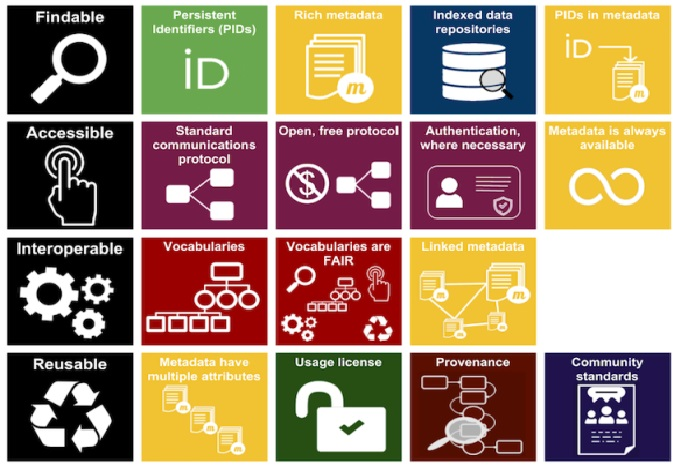
\includegraphics[width=0.8\linewidth,]{images/FAIR_data_principles2} 

}

\end{figure}

\hypertarget{dmp}{%
\section{DMP}\label{dmp}}

Los planes de manejo de datos (DMP) son una herramienta utilizada por la comisión europea (EC) para mejorar la producción y almacenamiento de datos producidos por investigaciones, consiste en una planificación respecto al ciclo de vida de los datos desde su creación hasta su preservación. En este sentido son una herramienta para la organización y estandarización del manejo de datos.

En un documento de apoyo para investigadores la \citet{ec_FAIR_2016} A modo de sintesis proponen documentar los siguientes puntos respecto al manejo de los datos

Componente DMP Problemas que deben abordarse

\begin{enumerate}
\def\labelenumi{\arabic{enumi}.}
\tightlist
\item
  \textbf{Resumen de datos}
\end{enumerate}

\begin{itemize}
\tightlist
\item
  Indique el propósito de la recopilación / generación de datos
\item
  Explicar la relación con los objetivos del proyecto.
\item
  Especificar los tipos y formatos de datos generados / recopilados
\item
  Especifique si los datos existentes se están reutilizando (si corresponde)
\item
  Especificar el origen de los datos
\item
  Indique el tamaño esperado de los datos (si se conoce)
\item
  Describa la utilidad de datos: para quién será útil
\end{itemize}

\begin{enumerate}
\def\labelenumi{\arabic{enumi}.}
\setcounter{enumi}{1}
\tightlist
\item
  \textbf{Datos FAIR}
\end{enumerate}

2.1. Haciendo que los datos se puedan encontrar, incluidos
disposiciones para metadatos

\begin{itemize}
\tightlist
\item
  Describir la capacidad de descubrimiento de datos (provisión de metadatos)
\item
  Resuma la identificabilidad de los datos y consulte el mecanismo de identificación estándar. ¿Utiliza identificadores persistentes y únicos como los identificadores de objetos digitales?
\item
  Esquema de convenciones de nomenclatura utilizadas
\item
  Describa el enfoque hacia las palabras clave de búsqueda
\item
  Describir el enfoque para versiones claras
\item
  Especificar estándares para la creación de metadatos (si los hubiera). Si no hay estándares en su
  disciplina describe qué tipo de metadatos se crearán y cómo
\end{itemize}

2.2 Hacer que los datos sean accesibles abiertamente

\begin{itemize}
\tightlist
\item
  ¿Especifique qué datos estarán disponibles abiertamente? Si algunos datos se mantienen cerrados, proporcione
  justificación para hacerlo
\item
  Especificar cómo estarán disponibles los datos
\item
  Especifique qué métodos o herramientas de software se necesitan para acceder a los datos. Es
  documentación sobre el software necesario para acceder a los datos incluidos? Es posible que
  incluir el software relevante (por ejemplo, en código fuente abierto)?
\item
  Especificar dónde están los datos y los metadatos asociados, la documentación y el código.
  depositado
\item
  Especifique cómo se proporcionará el acceso en caso de que haya restricciones
\end{itemize}

2.3. Hacer que los datos sean interoperables

\begin{itemize}
\tightlist
\item
  Evalúe la interoperabilidad de sus datos. Especifique qué vocabularios de datos y metadatos,
  estándares o metodologías que seguirá para facilitar la interoperabilidad.
\item
  Especifique si utilizará vocabulario estándar para todos los tipos de datos presentes en su
  conjunto de datos, para permitir la interoperabilidad interdisciplinaria? Si no es así, ¿proporcionará un mapeo para
  ontologías de uso más común?
\end{itemize}

2.4. Incrementar la reutilización de datos (mediante
aclarar licencias)

\begin{itemize}
\tightlist
\item
  Especificar cómo se licenciarán los datos para permitir la mayor reutilización posible
\item
  Especifique cuándo los datos estarán disponibles para su reutilización. Si corresponde, especifique por qué y
  por qué período se necesita un embargo de datos
\item
  Especificar si los datos producidos y / o utilizados en el proyecto son utilizables por terceros.
  fiestas, en particular después de la finalización del proyecto? Si la reutilización de algunos datos es
  restringido, explica por qué
\item
  Describir los procesos de aseguramiento de la calidad de los datos.
\item
  Especifique el período de tiempo durante el cual los datos permanecerán reutilizables
\end{itemize}

\begin{enumerate}
\def\labelenumi{\arabic{enumi}.}
\setcounter{enumi}{2}
\tightlist
\item
  \textbf{Asignación de recursos}
\end{enumerate}

\begin{itemize}
\tightlist
\item
  Estime los costos para hacer que sus datos sean FAIR. Describa cómo piensa cubrir estos
  costos
\item
  Identifique claramente las responsabilidades de la gestión de datos en su proyecto
\item
  Describir los costos y el valor potencial de la preservación a largo plazo.
\end{itemize}

\begin{enumerate}
\def\labelenumi{\arabic{enumi}.}
\setcounter{enumi}{3}
\tightlist
\item
  \textbf{Seguridad de los datos}
\end{enumerate}

\begin{itemize}
\tightlist
\item
  Abordar la recuperación de datos, así como el almacenamiento seguro y la transferencia de datos sensibles.
\end{itemize}

\begin{enumerate}
\def\labelenumi{\arabic{enumi}.}
\setcounter{enumi}{4}
\tightlist
\item
  \textbf{Aspectos éticos}
\end{enumerate}

\begin{itemize}
\tightlist
\item
  Para ser cubierto en el contexto de la revisión de ética, sección de ética de DoA y ética
  entregables. Incluya referencias y aspectos técnicos relacionados si no están cubiertos por el
  ex
\end{itemize}

\begin{enumerate}
\def\labelenumi{\arabic{enumi}.}
\setcounter{enumi}{5}
\tightlist
\item
  Otro
\end{enumerate}

\begin{itemize}
\tightlist
\item
  Consulte otros procedimientos nacionales / financiadores / sectoriales / departamentales para la gestión de datos.
  que está usando (si corresponde)
\end{itemize}

\hypertarget{rise-ddc-autoevaluaciuxf3n-para-el-proveedores-de-repositorios-abiertos.}{%
\section{RISE-DDC: Autoevaluación para el proveedores de repositorios abiertos.}\label{rise-ddc-autoevaluaciuxf3n-para-el-proveedores-de-repositorios-abiertos.}}

La organización del Reino Unido \href{https://www.dcc.ac.uk/}{Digital Curation Center DCC} es un centro de Curatoría digital, que nació el 2004 y tenía inicialmente el objetivo de apoyar en el almacenamiento de datos a nivel nacional. Posteriormente se ha masificado internacionalmente. Este centro ofrece servicios de Curatoría de distinto tipo, entre ellos asesoramiento técnico y programas de formación. Entregan información gratuita para ayudar a los centros de investigación y a las universidades en el almacenamiento de datos siguiendo los principios FAIR. En esta línea, la página web ofrece un marco de autoevaluación de la infraestructura de investigación \href{https://www.dcc.ac.uk/guidance/how-guides/RISE}{RISE} \citep{ddc_Using_2017}. El marco RISE describe 21 capacidades, distribuidas en diez áreas de servicio de soporte de datos de investigación (RMD, \emph{research data managament}).

\begin{figure}[!ht]

{\centering 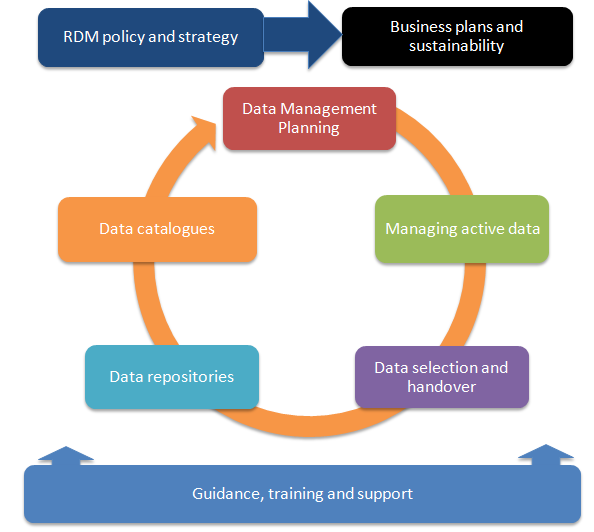
\includegraphics[width=0.8\linewidth,]{RDMcomponents} 

}

\caption{Propuesta RISE-DDI}\label{fig:unnamed-chunk-22}
\end{figure}

Los 21 puntos sobre estas 10 áreas se dividen en tres niveles, siendo cada uno mejor que el anterior. En general la lógica de los niveles va desde, lo más mínimo es cumplir con los requisitos del financiador (p.~ej. CONICYT) y lo máximo es establecerse como referente del campo en la apertura de datos. A continuación presentamos los aspectos generales sobre este esquema de autoevaluación de infraestructura para el soporte de datos.

\textbf{Política y estrategia}

Política de desarrollo: Las políticas institucionales que inciden en el RDM (por ejemplo, ética, investigación, etc.) están unidas y son complementarias. Las políticas se promueven externamente, con el objetivo de impulsar el sector, cumplen con los requisitos del financiador y fomentan el almacenamiento perdurable.

En particular, considerando el contexto de las CCSS, puede ser útil promover como política institucional de investigación a la ciencia abierta, fomentando materiales, análisis y publicaciones de investigación. También se puede poseer una política ética que, pese a la apertura, respalde la identidad de los sujetos de estudio, como \citet{dennis_Privacy_2019} señala necesario en el marco de la apertura.

Sensibilización y participación de las partes interesadas: La institución promueve las políticas a través de canales diseñados para interactuar con los intereses específicos del personal, los estudiantes y los grupos de investigadores.

Hoja de ruta de la implementación de RMD: a hoja de ruta / estrategia busca derivar una ventaja competitiva del soporte RDM, satisfaciendo necesidades de la institución y los financiadores.

\textbf{Sustentabilidad}

\begin{itemize}
\item
  lograr mantener financiamiento para personal y soporte técnico.
\item
  Existe un rediseño importante de las funciones del personal, de acuerdo con el establecimiento de un servicio RDM. Asignando nuevas funciones a los trabajadores de la institución para soportar el servicio de RMD.
\item
  La institución invierte en infraestructura técnica para todos los aspectos del ciclo de vida de los datos de investigación, interoperando con herramientas y flujos de trabajo a nivel de grupo de investigación.
\item
  Los recursos disponibles permiten ofrecer servicios de RDM independientes y especializados junto con la provisión de soporte estándar (por ejemplo, servicio de modelado estadístico, servicio de visualización de datos o servicio de apoyo a investigadores para la apertura).
\end{itemize}

\textbf{Servicios}

Esta área cubre la provisión de asesoramiento en línea y presencial para investigadores que necesitan apoyo con un aspecto particular de la gestión de datos de su investigación.

La orientación se adapta significativamente a las necesidades específicas de los investigadores y el personal de apoyo de la institución. El contenido de la guía se hace público para ser referenciado externamente como buenas prácticas del sector.

Normalmente, la prestación de servicios de asesoramiento variará en capacidad según el contexto institucional y las prioridades estratégicas. Por lo tanto, puede ser útil anotar debajo de la mesa qué temas puede proporcionar el servicio en cada nivel. Los temas de asesoramiento incluyen los siguientes:
• Costo de subvenciones
• Consentimiento y datos abiertos
• Reutilización de datos
• Análisis de datos
• Selección de datos
• Preservación de datos
• Metadatos
• Minería de texto y datos
• Visualización

\textbf{Entrenamiento}

• ¿Qué objetivos pretende abordar el programa de formación, p.~Ej. qué capacidades del servicio se mejorarán:
• qué habilidades o competencias deben desarrollarse: Como habilidades necesarias se encuentra la capacidad de utilizar las plataformas necesarias para construir el almacenamiento, subir los datos y

• qué canales se utilizan para conectar al personal y los investigadores con oportunidades de capacitación

\begin{itemize}
\tightlist
\item
  La institución produce una importante cantidad de material de formación online que satisface las necesidades de sus investigadores y personal. Los materiales son reutilizados por otras personas del sector.
\end{itemize}

Cabe destacar, que si es que se quiere contar con un menor gasto en servicios y personal administrando la curatoría de datos, es necesario que los investigadores posean una mayor capacitación para disminuir la necesidad del mejoramiento de la calidad de los datos.

\textbf{Plan manejo de datos}

Planificación de la gestión de datos. Esta área cubre el apoyo en línea y presencial para que los investigadores planifiquen eficazmente el componente de datos de su investigación y produzcan la documentación asociada.

Parte de esta documentación a ser producida refiere a los criterios con los que se selecciono la muestra y como se accedió a los sujetos (Ficha técnica), pauta de preguntas de la entrevista o cuestionario de la encuesta y manual de usuario.

La institución promueve las mejores prácticas en la planificación de la gestión de datos y facilita un buen diseño de investigación en relación con la generación y conservación de datos.

El servicio proporciona acceso automatizado a almacenamiento adicional para satisfacer demandas de rendimiento o capacidad excepcionales.

\textbf{Gestión activa de datos}

Abarca los servicios centrales, especialmente el almacenamiento y la sincronización de archivos.

¿Cómo se podría mejorar el soporte de gestión de datos mediante la integración del almacenamiento con otros sistemas relevantes? • ¿Cómo utilizan los investigadores los servicios en la nube de terceros? ¿Deben competir y / o integrar los servicios internos?

Sincronización y adaptabilidad:
El servicio proporciona acceso automatizado a almacenamiento adicional para satisfacer demandas de rendimiento o capacidad excepcionales.

Soporte de colaboración: El servicio proporciona acceso administrado a entornos de investigación virtuales que permiten a los investigadores trabajar con datos con colaboradores externos. Permite compartir datos con colaboradores externos. (no es muy aplicable en contexto de Open Data)

Manejo de la seguridad: El servicio proporciona herramientas / entornos que permiten a los investigadores des identificar, cifrar o controlar el acceso a los datos según sea necesario. Ojala cumplir las normas de seguridad digital ISO 27001/2

\textbf{Valoración y evaluación de riesgos}

\begin{itemize}
\item
  Qué ofrecerá el servicio a los investigadores para persuadirlos de que entreguen datos y metadatos.
\item
  Apoyo a la colaboración: Cómo se ayudará a los investigadores a identificar repositorios de terceros relevantes
\item
  Política de acumulación de datos: El servicio define los criterios para retención de conjuntos de datos de valor a largo plazo para la institución.
\item
  Apoyo legal/ técnico a investigadores: El servicio se compromete a gestionar de forma proactiva los riesgos legales y éticos relevantes para sus depositantes y usuarios, y al desarrollo profesional y técnico relevante para los investigadores y el personal de apoyo.
\item
  Metadatos: Los metadatos sobre los datos y los resultados de la investigación relacionados están lo suficientemente bien estructurados y son interoperables para permitir que se extraiga valor agregado para las necesidades de los usuarios del servicio.
\end{itemize}

\textbf{Preservación}

Esta área aborda la necesidad de garantizar la integridad y el acceso a los datos. Qué política y orientación se debe implementar para capturar la información contextual que otros necesitarán si quieren reutilizar los datos.

Planificación y acción de preservación: El servicio se compromete a implementar herramientas y experiencia para mantener las propiedades importantes de los datos, metadatos e información relacionada durante los períodos de retención requeridos e identificados grupos de usuarios.

Soporte continuo: El servicio permite que los datos y metadatos se distribuyan automáticamente en múltiples ubicaciones de acuerdo con criterios de políticas específicos.

\textbf{Acceso y publicación}

Esta área cubre el soporte para el depósito y publicación de datos de acceso abierto de valor a largo plazo. Algunos puntos a considerar son:

• ¿El contexto institucional garantiza el desarrollo de un repositorio de datos institucional?
• ¿Cómo debería integrarse un repositorio institucional con otros sistemas institucionales y externos?

Monitoreo de conjuntos de datos producidos localmente: Los metadatos sobre datos de investigación producidos localmente, y sus vínculos con otras actividades o productos, están suficientemente estructurados y organizados para informar la estrategia institucional.

Mandato de publicación de datos: El servicio respalda las necesidades de detección de contenido, acceso y revisión de calidad a medida para grupos de usuarios u organizaciones.

Nivel de curación de datos: El mínimo es la breve supervisión de la calidad de los datos y los metadatos. El óptimo es comprometerse a mejorar la calidad de los datos según las exigencias de cada proyecto.

\textbf{Descubrimiento}

Esta área se refiere a los procesos y mecanismos para recopilar y exponer los metadatos necesarios para que otros, dentro y fuera de la institución, averigüen qué datos producen sus investigadores, si son accesibles y dónde se guardan.

• Qué metadatos para los datos de investigación define la institución como ``esenciales'' y cómo se relaciona esto con los estándares relevantes para otros resultados de la investigación.

• Qué tan bien se integra un catálogo de datos con otros sistemas para la gestión y el descubrimiento de metadatos

Alcance de catalogación de metadatos: El servicio cataloga los metadatos para mejorar la reutilización potencial de conjuntos de datos de acuerdo con los estándares líderes del sector, o cumplir con propósitos específicos de dominio.

\hypertarget{oais-managament-research-data.}{%
\section{OAIS Managament Research Data.}\label{oais-managament-research-data.}}

Este documento es una práctica técnica recomendada para su uso en el desarrollo de un consenso más amplio sobre lo que se requiere para que un archivo proporcione una conservación permanente o indefinida a largo plazo de la información digital \citep[p.3]{ccsds_Recommendation_2012}. la CCSDS propone un marco común de términos y conceptos que componen un sistema de información de archivo abierto (OAIS). Un OAIS es un Archivo, que consiste en una organización, que puede ser parte de una organización más grande, de personas y sistemas que han aceptado la responsabilidad de preservar la información y ponerla a disposición de una Comunidad Designada (P.11).

Este documento no asume ni respalda ninguna plataforma informática específica, entorno de sistema, paradigma de diseño de sistema, metodología de desarrollo de sistema. Sino que plantea las obligaciónes para la preservación independiente del modo en que sera almacenado.

Esta subsección establece responsabilidades obligatorias que una organización debe cumplir en para operar un Archivo OAIS.

La OAIS deberá:
- Negociar y aceptar la información adecuada de los Productores de información.

\begin{itemize}
\item
  Obtener un control suficiente de la información proporcionada al nivel necesario para garantizar preservación a largo plazo.
\item
  Determinar, ya sea por sí mismo o en conjunto con otras partes, qué comunidades
  debe convertirse en la Comunidad Designada y, por lo tanto, debe poder
  comprender la información proporcionada, definiendo así su Base de Conocimientos.
\item
  Asegurarse de que la información a conservar sea comprensible de forma independiente para el
  Comunidad designada. En particular, la Comunidad Designada debería poder
  comprender la información sin necesidad de recursos especiales como la asistencia de
  los expertos que produjeron la información.
\item
  Siga políticas y procedimientos documentados que aseguren que la información sea
  preservado contra todas las contingencias razonables, incluida la desaparición del Archivo,
  asegurándose de que nunca se elimine a menos que se permita como parte de una estrategia aprobada. Allí
  no debe haber eliminaciones ad-hoc.
\item
  Poner la información preservada a disposición de la comunidad designada y habilitar
  la información que se difundirá como copias de, o como rastreable a, el original
  presentó objetos de datos con evidencia que respalde su autenticidad.
\end{itemize}

En el caso de las ciencias sociales la comunidad designada es, principalmente, el conjunto de investigadores de las ciencias sociales. Tambien podria ser el publico en general. Centrandonos en los investigadores parece razonable la necesidad de incluir la documentación necesaria para los datos publicados puedan ser debidamente comprendidos sin la necesidad de recurrir a quienes los crearon.

\begin{figure}
\centering
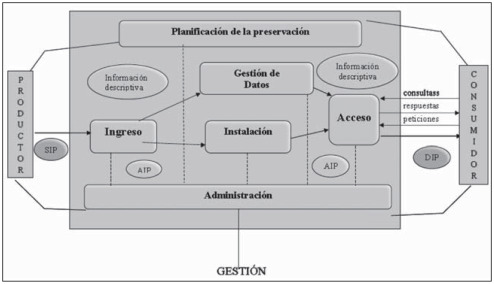
\includegraphics{EntidadesFuncionalesOAIS.JPG}
\caption{EntidadesF uncionales OAIS}
\end{figure}

\begin{itemize}
\tightlist
\item
  señalar las luces y sombras planteadas por \url{https://www.sciencedirect.com/science/article/pii/S0187358X16300545}
\end{itemize}

el objetivo principal es superar le problema de la rapida opsolecencia de los datos por cambios en elmundo digital.
- Oais es un esquema de preservacion digital creado

Otra propuesta similar de pasos a seguir para mejorar la calidad de los datos en miras de su apertura se encuentra en el segundo capítulo del libro ``Managament and sharing research data'' \citep{corti_Managing_2019}. Esta sección pone énfasis en los ciclos de vida de los datos, ciclo el cual debe ser comprendido como un proceso de producción y preparación de los datos que parte antes del levantamiento y termina después de publicados los resultados. Este conjunto de actividades ha sido elaborado en base a al Open Archival Information System (OAIS).

\begin{itemize}
\tightlist
\item
  Descubrimiento y planificación

  \begin{itemize}
  \tightlist
  \item
    Diseño de la investigación
  \item
    Planificación de la gestión de datos
  \item
    Planificación del consentimiento informado que permita abrir la información.
  \item
    Planificación de la recopilación de datos, protocolos de procesamiento y plantillas
  \item
    Exploración de las fuentes de datos existentes
  \end{itemize}
\item
  Recolección de datos

  \begin{itemize}
  \tightlist
  \item
    Recopilación de datos: registro, observación, medición, experimentación y simulación
  \item
    Capturar y crear metadatos
  \item
    Adquirir datos de terceros existentes
  \item
    Ingresar datos, digitalizar, transcribir y traducir.
  \item
    Verificar, validar, limpiar y anonimizar datos cuando sea necesario
  \end{itemize}
\item
  Procesamiento y análisis de datos

  \begin{itemize}
  \tightlist
  \item
    Describir y documentar datos
  \item
    Analizar e interpretar datos
  \item
    Producir resultados de investigación
  \item
    Creación de publicaciones
  \item
    Citar fuentes de datos
  \item
    Gestión y almacenamiento de datos
  \item
    Establecimiento de derechos de autor de los datos
  \end{itemize}
\item
  Publicación y uso compartido

  \begin{itemize}
  \tightlist
  \item
    Comprender otros derechos de propiedad intelectual de los datos
  \item
    Creación de metadatos de descubrimiento y documentación del usuario
  \item
    Selección del acceso apropiado a los datos Publicación / intercambio de datos
  \item
    Promoción de datos
  \item
    Migración de datos al mejor formato y medio
  \end{itemize}
\item
  Conservación de datos

  \begin{itemize}
  \tightlist
  \item
    Almacenamiento y copia de seguridad de datos
  \item
    Creación de documentación y metadatos de preservación
  \item
    Conservación y conservación de datos
  \item
    Realización de análisis secundarios
  \end{itemize}
\item
  Reutilización de datos

  \begin{itemize}
  \tightlist
  \item
    Realización de investigaciones de seguimiento
  \item
    Realización de revisiones de investigaciones
  \item
    Escrutinio de hallazgos
  \item
    Uso de datos para la enseñanza y el aprendizaje
  \end{itemize}
\end{itemize}

Además de esta lista de tareas para el ciclo de vida de los datos, se destaca la importancia de mantener los datos en un formato y una plataforma que faciliten el acceso a los datos en el futuro. También se destaca la importancia del control de versiones, sobre este punto y basados en las herramientas disponibles actualmente se considera optimo el uso de \href{https://github.com/}{Github} para el versionamiento de las bases de datos, pues esta página genera un registro de las distintas versiones y permite ir guardando los cambios cuando se considere necesario. Otra Herramienta que puede servir para investigadores menos experimentados es \href{https://openrefine.org/}{OpenRefine}, plataforma que fue diseñada por Google y está enfocada en la edición de bases de datos, permitiendo recodificaciones y transformaciones varias, además de mantener un registro de las versiones.

\hypertarget{tuberia-de-datos-icpsr}{%
\section{Tuberia de datos (ICPSR)}\label{tuberia-de-datos-icpsr}}

Una de las organizaciones mundiales más grandes en torno al almacenamiento de datos es Inter-university Consortium for Political and Social Research (ICPSR). Esta plataforma, además de dedicarse al almacenamiento de datos realiza cursos sobre curatoría de datos. Esta plataforma posee múltiples bases de datos de distintas áreas y ofrece la posibilidad de distintos servicios como la posibilidad de descargar el metadata, de realizar análisis en línea, de realizar gráficos y, además, posee herramientas para solicitar bases de datos con información sensible, para lo cual es necesario entregar una serie de documentos como el cv. Esta plataforma si bien ofrece estos servicios no todas las bases de datos los utilizan.

Esta organización, hace un tiempo realizo un curso sobre curatoría y mantenimiento de datos, curso en el cual se enseñó, entre otros conocimiento y herramientas, el diseño de flujo de datos ``tubería de procesamiento'', que es un esquema con los pasos necesarios para la publicación de los datos en línea. Los pasos de este esquema se encuentran en el siguiente esquema.

\begin{figure}[!ht]

{\centering 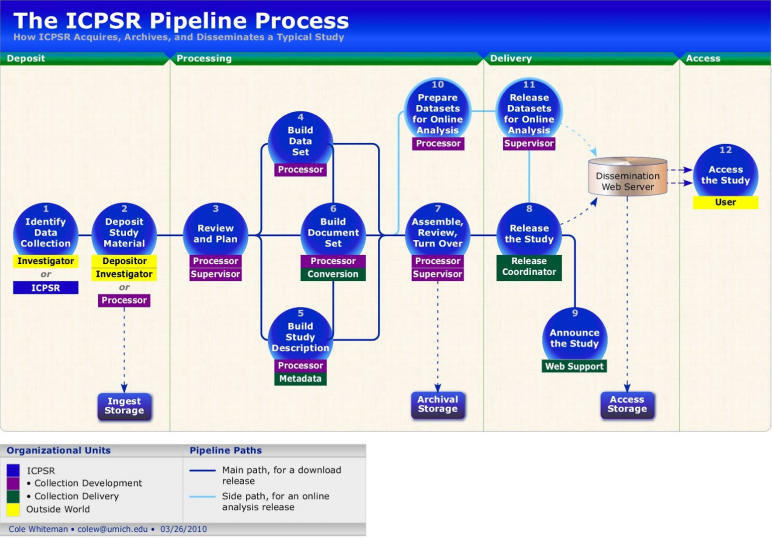
\includegraphics[width=0.8\linewidth,]{pipeline-ICPSR} 

}

\caption{Propuesta ICPSR}\label{fig:unnamed-chunk-23}
\end{figure}

De este esquema podemos destacar los siguientes puntos:

\begin{itemize}
\item
  Es importante la recolección del material asociado a la base de datos.
\item
  Es necesario construir metadatos suficientes.
\item
  Se sugiere abrir la posibilidad de datos en línea, los cuales deben ser supervisados para garantizar su continuo funcionamiento
\item
  Es conveniente guardar los datos ya procesados en una memoria local.
\item
  La difusión es fundamental como parte del proceso.
\end{itemize}

\hypertarget{esquema-cilac}{%
\section{Esquema (CILAC)}\label{esquema-cilac}}

Esta última organización ha generado un reporte para tomadores de decisiones, en el cual señala los logros y las barreras con los que se ha enfrentado el proceso de apertura de los datos de investigación.

para la presentación de datos, principios los cuales promueven también los documentos del caso chileno y europeo.

\textbf{INTRODUCIR GRAFICO}

\begin{figure}[!ht]

{\centering 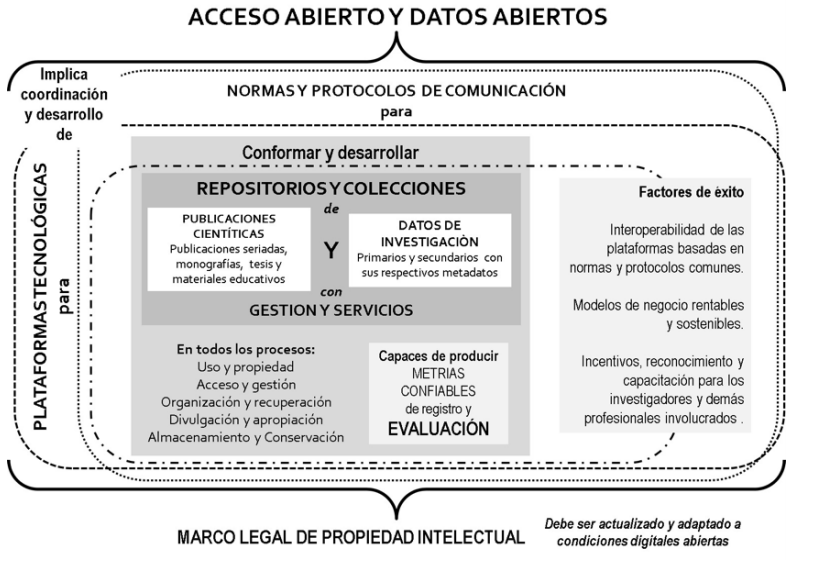
\includegraphics[width=0.8\linewidth,]{esquemacilac} 

}

\caption{Propuesta CILAC}\label{fig:unnamed-chunk-24}
\end{figure}

\textbf{Analizar gráfico}

Este grafico, a lo dicho anteriormente y en linea con RISE, un centro o politica de almacenamiento abierto require de generar información metrica sobre la cantidad de registros y permita procesos de evaluación.

\hypertarget{experiencias-sobre-el-almacenamiento-de-datos-de-investigaciuxf3n}{%
\chapter{Experiencias sobre el almacenamiento de datos de investigación}\label{experiencias-sobre-el-almacenamiento-de-datos-de-investigaciuxf3n}}

En el presenta apartado presentamos un conjunto de repositorios digitales de materiales de investigación. Se realizaran comentarios, evaluaciones y destacaran aportes de estos repositorios digitales. Para ordenar su presentación primero revisaremos quellas experiencias internacionales que han destacado como las mejores en el ambito. Luego veremos algunas experiencias a nivel latinoamericano y chileno, para evaluar sus fortalezas y debilidades en base a los criterios y estándares presentados en la sección anterior.

\hypertarget{existosos-repositorios-internacionales}{%
\section{Existosos repositorios internacionales}\label{existosos-repositorios-internacionales}}

\hypertarget{icpsr}{%
\subsection{ICPSR}\label{icpsr}}

Este es un consorcio internacional de más de 750 instituciones académicas y organizaciones de investigación, el Consorcio Interuniversitario de Investigación Política y Social (ICPSR) proporciona liderazgo y capacitación en acceso a datos, curación y métodos de análisis para la comunidad de investigación en ciencias sociales.

ICPSR mantiene un archivo de datos de más de 250.000 archivos de investigación en las ciencias sociales y del comportamiento. Alberga 21 colecciones especializadas de datos en educación, envejecimiento, justicia penal, abuso de sustancias, terrorismo y otros campos.A continuación se presenta una visualización de un ejemplo dos ejemplos de datos de este repositorio.

El ejemplo que se presenta a continuación posee como propósito comprender mejor el problema de la agresión sexual entre las mujeres afroamericanas en Maryland Estados Unidos , evaluar el uso de los recursos disponibles en respuesta a la agresión sexual y explorar el uso de fuentes alternativas de atención \citep{weist_African_2009}. Los investigadores entrevistaron a 223 mujeres víctimas de agresión sexual (Parte 1 y Parte 2) entre enero de 2004 y julio de 2005 y realizaron 21 grupos focales (Parte 3). A continuación puede ver la pagina web para observar los recursos que posee.

Como puede verse se ofrece al usuario una descripción general del documento, lo cual facilita a los investigadores evaluar la pertinencia de su uso. Tambien se puede descargar la documentación y los datos del estudio, pero dado la tematica y la importancia de ser prudentes con su divulgación estos deben solicitarse explicando el uso investigativo que se dará para que los autores evaluen si se dara acceso a los datos.

En terminos FAIR este documento poseee un identificador, es encontrable y esta en un fomrato que es ampliamente utilizado el pdf. No obstante quizas seria bueno que las entrevistas tambien esten en formato de texto plano txt, para garantizar su perdurabildiad al largo plazo.

La siguiente base de datos trabaja sobre el desarrollo de los adolecentes y cuenta con más de 10 olas \citep{mortimer_Youth_2009}. Adempas a sido descargadad más de 100 mil veces, y posee más de 209 publicaciónes asociadas, lo que da cuenta de la buena difución con la que ha contado esta base datos y su posibilidad de ser usada por otros investigadores. Le invitamos a revisar los componentes en el repositorio.

Un problema frecuente con los metadatos es que se requiere utilizar un formato de metadatos en particular, formato que no siempre acomoda a todos quienes requieran de ellos y además cambien en el tiempo \citep{gomez_Datos_2016}. Al respecto esta pagina posee como ventaja que permite al usuario descargar los metadatos en distintos formatos.

Evaluado desde el punto de vista FAIR, podemos decir que cumple en buena medida los criterios, posee un identificador incluido en los metadatos que ademas tiene un protocolo de comunicación estandarizado (``http//''). Si bien en este documento se puede acceder directamente a los materiales, en otros proyectos de ICPSR se requiere autorización para ello, lo cual da cuenta de lo diámico y flexible de la plataforma.

Para descargar los datos se debe generar una cuenta que puede ser un usuaro asociado a un correo, una cuenta google, linkenid o ocid. Es bastante sensillo y rapido generar la cuenta para descargar los datos. Al hacerlo se nos adbierte las condiciones de uso y la licencia con la que cuenta la base de datos lo cual esta en linea con Fair.

En terminos de interoperabilidad al descargar la base de datos se pueden elegir entre multiples fomratos para los datos lo cual facilita su uso por distintos investigadores.

No obstante sus buenos estandares de almacenamiento, no se puede acceder a los datos de esta investigación si no se es miembro de una orgnaizaicon en alianza con ICPSR.

Un aspecto destacable respecto a este repositorio es que posee una pestaña donde se pueden encontrar todos las publicaciones relacionadas con este conjunto de datos, lo cual fomenta la colaboración y ayuda a eliminar la ineficiente practica de ``Reinventar la rueda''.

\begin{verbatim}
  Evaluar segun el resto de los parametros. 
  
  
  Diccionario sobre temas de almacenamiento de datos para cientiestas sociales. 
  https://www.icpsr.umich.edu/web/ICPSR/cms/2042  Documentación es un termino adecuado.     
  
  https://www.icpsr.umich.edu/files/ICPSR/curation/preservation/policies/dp-policy-outline.pdf 
  gia de politicas
\end{verbatim}

\hypertarget{qualitative-data-repository}{%
\subsection{Qualitative Data repository}\label{qualitative-data-repository}}

El repositorio de datos cualitativos (QDR) es un archivo dedicado para almacenar y compartir datos digitales (y la documentación adjunta) generados o recopilados a través de la investigación cualitativa y de múltiples métodos en las ciencias sociales. QDR proporciona servicios de consultoría en gestión de datos y selecciona activamente todos los proyectos de datos, manteniendo el valor y la utilidad de los datos a lo largo del tiempo y asegurando su disponibilidad y posibilidad de encontrarlos para su reutilización.

A continuación, se presenta una página web ya referenciada en este documento sobre la participación de género en el desarrollo comunitario en torno a los fondos climáticos de descentralización. Este trabajo ofrece un conjunto de documento como las pautas de Focus Groups y sus transcripciones, aunque solo se tiene de libre acceso las pautas y para acceder a las transcripciones se requiere una cuenta y solicitarlas a los investigadores responsables mediante la página. Si gusta puede revisar dicho contenido en el siguiente \href{https://data.qdr.syr.edu/dataset.xhtml?persistentId=doi:10.5064/F6HTXF0H}{link}

Este repositorio cuenta con un identificador indicado en metadatos contundentes que además están indexados en un buscador web. También poseen un protocolo de comunicación estandarizado, además de poseer medios para la autorización del uso del material.

Además, la página facilita el uso permitiendo previsualizaciones de los documentos que se encuentra abiertos, recurso que se encuentra igualmente en los otros buenos ejemplos de repositorios de datos.

Otra temática importante que es trabajada por este repositorio es su apoyo en el hacer anónimos los datos, lo cual da cuenta de un compromiso por resguardar la seguridad de los investigadores y apoyarles como sugiere necesario el documento de Autoevaluación RISE.

En vista de que los datos son accesibles si se los solicita, y considerando la importancia ética de generar consentimientos informados coherentes con la ciencia abierta \citep{dennis_Privacy_2019}, se puede hacer una crítica al hecho de que el consentimiento informado en el estudio no explicita a los sujetos de investigación que las entrevistas se pondrán a disposición de la comunidad científica mediante solicitud.

Como aspectos positivos esta página también cuenta con la posibilidad de exportar los metadatos en distintos formatos ampliamente reconocidos como DC, DDI, JSON.

Respecto a los factores de éxito señalados por CILAC, se señala la importancia de los incentivos para los investigadores. Entre estos incentivos el reconocimiento y las citas son importantes. Al respecto el repositorio expuesto posee pocas descargas (88) y ninguna cita, esto podría ser eventualmente un problema de difusión.

\hypertarget{uk-data-service}{%
\subsection{UK Data Service}\label{uk-data-service}}

El Servicio de Datos del Reino Unido está financiado por el Consejo de Investigación Económica y Social (ESRC) para satisfacer las necesidades de datos de investigadores, estudiantes y profesores de todos los sectores, incluidos el mundo académico, el gobierno central y local, organizaciones benéficas y fundaciones, centros de investigación independientes, grupos de expertos, y consultores empresariales y del sector comercial.

La recopilación del Servicio de datos del Reino Unido incluye las principales encuestas patrocinadas por el gobierno del Reino Unido, encuestas transnacionales, estudios longitudinales, datos del censo del Reino Unido, agregados internacionales, datos comerciales y datos cualitativos.

Esta página también logra satisfacer los principios Fair. En términos del repositorio estos también se adaptan a los criterios de autoevaluación RISE, en los cuales se señala a la importancia de generar apoyo a los usuarios, acción realizada por el UK Service para sus miembros.

Para acceder a los datos se requiere una cuenta registrada, la cual solo es para personas que son parte de las organizaciones afiliadas al repositorio.

\hypertarget{dataverse-harvard}{%
\subsection{Dataverse Harvard}\label{dataverse-harvard}}

El Proyecto Dataverse es una aplicación web de código abierto para compartir, preservar, citar, explorar y analizar datos de investigación. Facilita la puesta a disposición de otros de los datos y le permite replicar el trabajo de otros con mayor facilidad. Los investigadores, las revistas, los autores de datos, los editores, los distribuidores de datos y las instituciones afiliadas reciben crédito académico y visibilidad en la web.

De este modo, dataverse no solo apoya el proceso de almacenamiento de matariales e información para la investigación sino que tambien posibilita el almacenamiento de codigos para la reproducibilidad, comprendida como la posibilidad de volver a ejecutar un analisis con los mismos datos y mismos procedimientos usualmente especificados en codigos.

Un repositorio de Dataverse es la instalación del software, que luego aloja varios archivos virtuales llamados colecciones de Dataverse. Cada colección de Dataverse contiene conjuntos de datos, y cada conjunto de datos contiene metadatos descriptivos y archivos de datos (incluida la documentación y el código que acompañan a los datos). Como método de organización, las colecciones de Dataverse también pueden contener otras colecciones de Dataverse.

Segun la institución, la idea central detrás del Proyecto Dataverse es automatizar gran parte del trabajo del archivero profesional y proporcionar servicios y distribuir crédito al creador de datos. Antes del Proyecto Dataverse, los investigadores se vieron obligados a elegir entre recibir crédito por sus datos, controlando la distribución ellos mismos pero sin garantías de conservación a largo plazo, o tener garantías de conservación a largo plazo, enviándolos a un archivo profesional pero sin recibir mucho crédito. El Proyecto Dataverse rompe esta mala elección: colocamos una colección de Dataverse (un archivo virtual) en su sitio web que tiene el aspecto, la sensación, la marca y la URL de su sitio web, junto con una cita académica para los datos que le brindan crédito y visibilidad web completos.

El siguiente es un ejemplo de conjunto de datos sobre la replicación de un estudio sobre lasa actitudes de los residentes urbanos hacia la migración ambiental en Kenia y Vietnam.

Evaluando este conjunto de datos desde la perspectiva Fair podemos decir que es un buen ejemplo y cumple con los requisitos.

Un aspecto destacable de este repositoro es que poseen un previsualizador de los datos, asi como un espacio para observar las distintas versiones de los archivos.

\hypertarget{gesis}{%
\subsection{GESIS}\label{gesis}}

Gesis es actualmente la institión con mayor infraestructura para CCSS de alemania. Ofrece una gran cantida dde servicios de acceso a datos de invesitgaciónes, publicaciones, instrumentos de medición entre otros.

\citet{europeancommissionbrussels_Flash_2015}

\hypertarget{repositorio-en-osf}{%
\subsection{REPOSITORIO EN OSF,}\label{repositorio-en-osf}}

Open Science Framework (OSF) es una plataforma con la intención de centralizar las labores de almacenamiento e infraestructura digital que son necesarios para las distintas etapas del proceso investigativo. Esta página está hecha para almacenar hipótesis, diseños de investigación, bases de datos, resultados y versiones de los artículos o publicaciones finales. Esta plataforma puede ser utilizada gratuitamente por cualquier usuario, lo que permite a los investigadores concentrarse en investigar y dejando estas funciones a la plataforma.

Si se poseen recursos de una institución y sus participantes lo desean, pueden contratar un servicio espacial de OSF que permite hacer páginas web de los distintos proyectos de investigación de una institución, vinculando estos proyectos entre sí. A continuación, se expone una página que Almacena investigaciones de a2jLab un laboratorio de acceso a la justicia. Puede acceder al repositorio mediante el siguiente \href{https://osf.io/institutions/a2jlab/}{link}

Si bien las investigaciones depositadas no utilizan todos los recursos, se puede apreciar que es posible crear un conjunto de recursos de distinto tipo adecuados para la investigación social. Por ejemplo, la plataforma permite hacer pre-registros para investigaciones cuantitativas y cualitativas. Los pre-registros implican exponer con anterioridad las hipótesis que se poseen antes de hacer el análisis de los datos, para evitar que se generen hipótesis a posteriori señalando engañosamente que fueron pensadas teóricamente anteriores al análisis de la información.

Como aspecto negativo se debe señalar que si bien la página genera identificadores únicos que pueden servir tanto para los artículos como para las bases de datos y se poseen metadatos, estos últimos son bastante restringidos. No se pueden agregar nuevas celdas de información para los metadatos ni se pueden exportar a distintos estándares de metadatos.

\hypertarget{fragilefamilies}{%
\subsection{fragilefamilies}\label{fragilefamilies}}

Una experiencia en el almacenamiento de bases de datos es el centro de investigación ``Fragile Families'' que posee un repositorio abierto de su estudio longitudinal. Esta plataforma facilita la búsqueda de datos a los investigadores a partir de un \href{https://fragilefamilies.princeton.edu/data-and-documentation/metadata-explorer}{buscador de datos}. Este último muestra un resumen de las variables de cada ola de su estudio longitudinal como se puede observar en la imagen posterior. Considero que este es un valioso recurso que facilita a los investigadores la toma de decisiones respecto a los datos a utilizar.

\begin{figure}[!ht]

{\centering 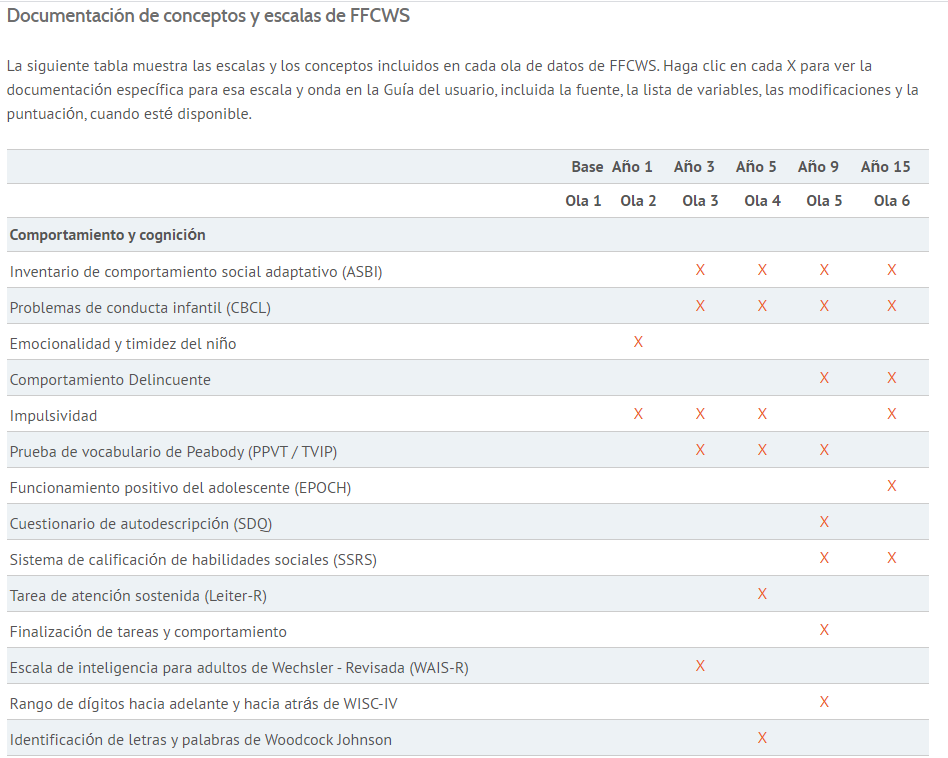
\includegraphics[width=0.8\linewidth,]{reslong} 

}

\caption{Tolerar ideas distintas es el valor más importante que debieran aprender}\label{fig:unnamed-chunk-25}
\end{figure}

\hypertarget{experiencia-regional.}{%
\section{Experiencia regional.}\label{experiencia-regional.}}

\hypertarget{lapop.}{%
\subsection{LAPOP.}\label{lapop.}}

Segun su propia pagina web \citep{lapop_Inicio_2020} LAPOP es la principal institución académica que realiza encuestas de opinión pública en las Américas, con más de 30 años de experiencia. Como centro de excelencia en investigación por encuestas, LAPOP usa enfoques y métodos innovadores con los ``estándares más altos'' para llevar a cabo encuestas nacionales; conducir estudios de evaluación de impacto, y producir reportes acerca de las actitudes, evaluaciones y experiencias de los individuos. El Barómetro de las Américas es la única encuesta comparativa y científicamente rigurosa que cubre 34 naciones incluyendo Norte, Centro y Sur América, así como también, un significativo número de países en el Caribe. Cada año publica docenas de estudios académicos de alta calidad y artículos de relevancia para la elaboración de políticas públicas.

Cabe destacar que si bien esta es una experiencia de almaceneamiento de datos para investigaciones posee algunas diferencias. Por ejemplo es una plataforma solo para almacenar encuestas del proyecto LAPOP y no asi de otras investigaciones afines. Por ello los servicios de clasificación de datos y priorizacion no son tan importantes por que no se posee un volumen tan grande de datos.

como se puede ver en la proyección de la pagina esta ordena las bases de datos en base a paises, ademas de tener otras entradas. Respecto a su adecuación a los estandares internacionales, se puede ver que no cumple con los parametro FAIR, ya que no posee un identificador único ni metadatos adecuados.

Como aspecto positivo las bases de datos cuantitativas son ofrecidos en dos de los formatos más utilizados SPSS y STATA. Tambien entragan documentacion fundamental para el trabajo con bases de datos como son los informes tecnicos y los cuestionarios. En terminos de facilitar el uso, no se entregan previsualizaciones de los datos, ni la posibilidad de graficar frecuencias, lo cual podria ser un aporte la democratización de los datos.

\hypertarget{plataforma-integrada-de-datos-del-mincyt-argentina}{%
\subsection{Plataforma integrada de datos del MINCYT Argentina}\label{plataforma-integrada-de-datos-del-mincyt-argentina}}

A partir de la información recopilada por el foro CILAC, se puede decir que en algunos países del continente los gobiernos están realizando esfuerzos por fomentar la apertura de los datos. Por ejemplo, en argentina, a partir de una nueva ley de Acceso abierto, se propuso una \href{http://datos.mincyt.gob.ar/}{plataforma integrada para el acceso a datos}. Esta plataforma entrega información sobre distintas disciplinas. Entre estos trabajos, el más cercano a las ciencias sociales son los \href{https://datasets.datos.mincyt.gob.ar/dataset/personal-de-ciencia-y-tecnologia/archivo/11dca5bb-9a5f-4da5-b040-28957126be18}{Datos de personal de ciencia y tecnologia}, que permite hacer análisis socioedmografico de los academicos. Esta plataforma posee una previsualización y una tabla con las variables que facilita el conocimiento de los datos, los cuales están disponibles para descargar distintos formatos. Esta previsualización se puede realizar a modo de tablas, gráficos y mapas. No obstante, la visualización mediante gráficos es relativamente ineficiente, puesto a que es difícil lograr gráficos que sean comprensibles.

En el informe de la CILAC, también se menciona el caso de Chile, Perú y México, pero ni una de las páginas de los ministerios de ciencia de estos países permite localizar las bases de datos con la que trabajaron los investigadores. Por dicho motivo este informe no ahondara en dichosos casos.

\hypertarget{cepal-stats}{%
\subsection{CEPAL stats}\label{cepal-stats}}

\url{https://estadisticas.cepal.org/cepalstat/Perfil_Regional_Economico.html?idioma=spanish}

\hypertarget{evaluaciuxf3n-de-experiencias-nacionales.}{%
\section{Evaluación de experiencias nacionales.}\label{evaluaciuxf3n-de-experiencias-nacionales.}}

Hace bastantes años que a nivel nacional se realizan esfuerzos por fomentar el registro abierto de datos. La antigua Comisión Nacional de Investigación Científica y Tecnológica (CONICYT), en la página \href{http://datoscientificos.cl/}{Datos Cientificos}\citep{programadeinformacioncientifica_Ciencia_2019}, realiza una propuesta de politica para datos abiertos. El primer punto de dicha propuesta exige a todos los beneficiarios de CONICYT la publicación de informes con datos producidos de la investigación. En favor de dicha política se publicaron el año 2010 y 2014 dos documentos con sugerencias para la apertura de los datos.

El primero de estos informes es una revisión del estado del arte de la accesibilidad de datos \citep{munoz_ESTADO_2010}. se destacan las siguientes recomendaciones.

\begin{itemize}
\item
  A partir de la experiencia de las Políticas de Intercambio de Datos Científicos en China se evidenció la dificultad de desarrollar una política nacional de gestión cuando en la cultura científica local persistió la idea de propiedad personal. Por ello, es fundamental realizar políticas de concientización respecto a los datos abiertos.
\item
  En base a la recopilación de datos epidemiológicos del National Center for Health Statistics de Estados Unidos, se releva la importancia de preparar alternativas para datos sensibles. Considerando la naturaleza de los datos, es necesario en algunas ocasiones mantener los datos en la mayor confidencialidad posible. En esta línea, la organización mencionada junto con dejar los datos de acceso abierto, mantuvieron algunos datos en privado a los cuales solo se puede acceder en base a una solicitud con una propuesta de investigación y mediante una plataforma que posibilita cálculos sin permitir el acceso directo a los datos ni su transferencia. Es fundamental identificar aquellas investigaciones que requieren un resguardo mayor de datos y generar protocolos para su uso.
\end{itemize}

El segundo documento, escrito el 2014, se denomina ``Datos Científicos Abiertos La Ciencia la hacemos entre todos, Programa de Información Científica'' \citep{hernandez_Manual_2014}. Este informe posee la intención de ser un manual respecto a cómo abrir los procesos investigativos. Se destacan las siguientes recomendaciones:

\begin{itemize}
\item
  Utilizar una licencia de Creative Commons: permiten autorizar el uso de terceros sin perder los derechos de atribución.
\item
  Utilizar repositorios interoperables: Para facilitar la recopilación automática de datos y el uso de estos desde distintos Software, se recomienda poseer buenos metadatos siguiendo los parámetros de interoperabilidad de \href{http://dublincore.org/}{Dublin Core}. Los metadatos son ``los datos sobre los datos'' es decir aquella información que nos permite saber a qué corresponde la base de datos, quienes y cuando la crearon entre otras informaciones relevantes. Esta página propone una decena de metadatos indispensables para la interoperabilidad (Ej. creador, colaborador, editor, título, fecha, idioma, formato, tema, descripción, identificador, relación, fuente, tipo, cobertura y derechos, entre otros) \citep{dublin-core_Dublin_2020}. Si bien esta publicación no da cuenta de que metadatos debe ser específicamente utilizado a partir de la información anterior producida por lisa podemos decir que es beneficioso utilizar el conjunto de metadatos para social-science que es un conjunto bastante parsimonioso de información.
\end{itemize}

Pueden observarse documentos que buscan la publicación abierta de las bases de datos desde varios años. Por ejemplo, (en esta pagina){[}\url{https://www.uchile.cl/portal/informacion-y-bibliotecas/servicios-de-biblioteca/bases-de-datos/57683/indice-por-tema}{]}. No obstante como puede verse en ese sitio aun no es posible encontrar a libre disposición los resultados y los materiales de las investigaciones dando cuenta de una buena politica que no ha sido terminada.

A, a las bases de datos de la Univercidad Diego Portales (UDP) y a la información nacional producida por el PNUD-Desiguales. Estas son buenas experiencias ya que poseen una amplia llegada a los investigadores siendo estas bases utilizadas por ellos. En vista de su popularidad y accesibilidad por parte de los usuarios, se observo el modo en que se hacen accesibles las bases llegando a los siguientes aprendisajes y sujerencias:

\hypertarget{cep}{%
\subsection{CEP}\label{cep}}

El Centro de Estudios públicos produce constantemente encuestas de opinión publica, con bastante contenido electoral. Esta es una de las bases de datos más conocidas en el campo de la sociología de Chile. Y en el último tiempo mejoro su plataforma de almacenamiento.

Ahora la página posee un buscador de datos, un espacio para descargar una base consolidada longitudinal con los distintos estudios y un recurso para realizar gráficos en línea, lo cual fomenta la utilización por el público no especializado. Además, como siempre, la página cuenta con material suficiente para utilizar las bases de datos como las fichas técnicas, documentos de resultados y las bases de datos en distintos formatos (SPSS, STATA y R). Respecto a las bases de datos es de las pocas bases de datos analizadas que codifico las etiquetas de la base de datos en UTF-8. Como aspectos negativos se puede señalar que no se cuenta con recurso para descargar metadatos ni posee un identificador único

incluir: casen, desiguales-pnud (no fairs)

\hypertarget{coes-dataverse}{%
\subsection{COES-Dataverse}\label{coes-dataverse}}

posee metadatos y doi. posee información necesaria para trabajar. permite almacenar distintos documentos.

Como aspecto positivo ofrece metricas sobre la descarga de los datos que permiten generar perfiles sobre el publico. Esto esta en linea con lo señalado por CILAC respecto a la construccion de metircas sobre los registros que permitan evaluación.

\hypertarget{movid.}{%
\subsection{Movid.}\label{movid.}}

En el corto plazo la experiencia de almacenamiento de datos relativos al covid es un caso interesante de aprovechar en términos de aprendizaje. \href{https://www.minciencia.gob.cl/covid19}{Datos Covid Ministerio de Ciencias}. Esta recopilación de los casos se guardó en la plataforma Github cuenta con un visualizador Shiny que permite a usuarios básicos en línea realizar análisis descriptivos sobre las variables.

En una línea similar el proyecto del \href{https://ocs-coes.netlify.app/app/}{observatorio de cohesión social} generado por COES, es una buena experiencia, no tanto en el almacenamiento de bases de datos sino en la visualización de los mismos la cual fomenta para la democratización del conocimiento.

  \bibliography{almacenamiento.bib}

\end{document}
